\documentclass[11pt,a4paper,onecolumn]{article}
\usepackage[T1]{fontenc}
\usepackage[utf8]{inputenc}
\usepackage{lmodern}
\usepackage[margin=23mm]{geometry}
\usepackage{microtype}
\usepackage{amsmath,amssymb}
\usepackage{graphicx}
\usepackage{xcolor}
\usepackage{array,booktabs,tabularx,longtable}
\usepackage{caption,subcaption}
\usepackage{enumitem}
\usepackage{placeins}
\usepackage{tikz,pgfplots}
\usetikzlibrary{arrows.meta,positioning,calc}
\pgfplotsset{compat=1.17}
\usepackage[hidelinks]{hyperref}
\usepackage{url}
\definecolor{ink}{HTML}{203447}
\definecolor{teal}{HTML}{227C80}
\definecolor{softgray}{HTML}{EDF1F4}
\definecolor{warm}{HTML}{B56B42}
\captionsetup{font=small,labelfont=bf,labelsep=period}
\setlist[itemize]{leftmargin=1.5em,itemsep=3pt,topsep=4pt}
\setlist[enumerate]{leftmargin=1.8em,itemsep=3pt,topsep=4pt}
\setlength{\parskip}{5pt plus 1pt}
\setlength{\parindent}{0pt}
\setlength{\tabcolsep}{4pt}
\renewcommand{\arraystretch}{1.17}
\renewcommand{\topfraction}{0.90}
\renewcommand{\textfraction}{0.08}
\renewcommand{\floatpagefraction}{0.75}
\setlength{\emergencystretch}{2em}
\raggedbottom
\newcolumntype{L}[1]{>{\raggedright\arraybackslash}p{#1}}
\newcolumntype{Y}{>{\raggedright\arraybackslash}X}
\newcommand{\artifact}[1]{\nolinkurl{#1}}
\newcommand{\na}{\textemdash}
\newsavebox{\methodologyoverviewbox}
\newsavebox{\compactresultstablebox}
\newenvironment{singlepagetable}{%
  \begin{lrbox}{\compactresultstablebox}\begin{minipage}{\linewidth}%
}{%
  \end{minipage}\end{lrbox}%
  \ifdim\dimexpr\ht\compactresultstablebox+\dp\compactresultstablebox\relax>\textheight
    \PackageError{GRASP-layout}{A compact results table exceeds one page}{Reduce table spacing without removing data.}%
  \fi
  \noindent\usebox{\compactresultstablebox}%
}

\pgfplotsset{every axis/.append style={label style={font=\small},tick label style={font=\small},legend style={font=\small,draw=none},axis line style={black!55},grid style={black!12},major tick length=2pt}}
\title{\textbf{GRASP: A Greenwashing Recognition and Scoring Pipeline\\for Structured BRSR Disclosures in India}}
\author{\normalsize Yugchhaya Galphat, Purab Keshwani, Khushi Dayaramani,\\
\normalsize Ronit Chugwani, and Karan Sarani\\[5pt]
\small Computer Department, Vivekanand Education Society's Institute of Technology\\
\small Mumbai, India\\[3pt]
\footnotesize yugchhaya.dhote@ves.ac.in; 2023.purab.keshwani@ves.ac.in\\
\footnotesize 2023.khushi.dayaramani@ves.ac.in; 2023.ronit.chugwani@ves.ac.in\\
\footnotesize 2023.karan.sarani@ves.ac.in}
\date{}
\begin{document}
\maketitle
\begin{abstract}
India's listed companies publish Business Responsibility and Sustainability Reports (BRSR) containing written explanations and numerical disclosures. Reviewing these reports requires analysts to organise the text, find supporting figures, and compare companies using a common scoring method. GRASP combines these tasks in a seven-module pipeline. Reports are first collected and stored with company, reporting-period, and measurement details. Reporting tags and concept mappings then assign principle labels automatically to selected text segments. These automatically assigned labels are called weak labels. A BERT language model is first adapted to BRSR language and then trained on the labelled text segments to recognise the nine reporting principles. Word lists and sentence similarity identify vague wording, while numerical and assurance checks create review records linked to reported evidence. Classifier probabilities also provide a report-level summary for each principle. A Transparency Score combines Completeness, Specificity, Clarity, and Sustainable Development Goal (SDG) breadth; Clarity reuses the vagueness detector. Sector comparisons and an application programming interface (API) make the outputs available for review. The saved application results cover 1,164 companies. On 6,201 text segments from 175 companies excluded from supervised training, the classifier achieves 93.00\% agreement with report-derived weak labels. Comparison with 20 historical human ratings gives a Pearson correlation of $r=0.6314$ for the Transparency Score. The workflow allows an analyst to move from company and sector summaries to the text segments, score components, and reported values behind each result.
\end{abstract}
\noindent\textbf{Keywords:} BRSR; sustainability disclosure; weak supervision; BERT; vagueness detection; transparency scoring; sector benchmarking.
\section{Introduction}
\label{sec:introduction}

 India's Business Responsibility and Sustainability Reporting (BRSR) framework gives environmental, social, and governance (ESG) disclosures a common structure. The Securities and Exchange Board of India (SEBI) made BRSR reporting mandatory in 2021 for the top 1,000 listed companies by market capitalisation, and the rule applies from financial year 2022--23. The framework rests on nine principles of responsible business conduct. Essential indicators must be reported, but leadership indicators are voluntary \cite{sebi2021}. Every year, each company files one complete document, called a \emph{report}. A common format makes reports easier to organise. The format alone, however, cannot show whether every answer is complete or correct.

Reviewing one report by hand is a slow job with several steps. The analyst first finds a \emph{text segment}, which is the selected portion of the report's text that is analysed, and places the text segment under a topic. Then the analyst looks for a related number. This number must be checked for the reporting year, the unit, and the part of the business that the number covers. Comparing companies adds more difficulty. Business activities differ, so different reporting items apply to each company. Across hundreds of reports, these steps take a great deal of time. Take the claim \emph{water use decreased} as an example. The claim can be assessed only after a matching water measure, the business boundary, and the comparison period are found.

Automated text analysis can reduce this workload. ClimateBERT finds climate-related language and some disclosure categories. ChatReport retrieves text from reports and answers reporting questions, with a link to the source for each answer. ESGReveal pulls structured information out of narrative reports \cite{webersinke2021,ni2023,zou2025}. Methods like these make large collections of reports easier to organise. Even so, three questions remain once a connected workflow is built for structured Indian reports.

Three questions are still open. The first is \emph{how to connect a claim with evidence}. A phrase detector can find a promise, and a text-similarity model can tell that a sentence is about the environment. Neither tool checks the number behind the sentence. That number must fit the meaning of the claim, the reporting period, and the reporting context before the number counts as support.

The next question is \emph{how to organise training labels}, meaning the correct answers from which a model learns. Labelling every text segment by hand would be slow. Tags and concept maps in the report offer a repeatable alternative, and the source of each label is recorded for every text segment.

The last question is \emph{how to interpret a company score}. A score means little unless the reader knows how the score was produced. This requires stating the calculation, the items included, the sector group, and the reference source. GRASP brings these requirements together in one connected BRSR workflow with clearly defined tests \cite{calamai2025,garg2025}.

Each of these questions gets a direct answer in GRASP. For the link between claim and evidence, text segments and structured facts sit under the same report. A \emph{fact} is one reported value together with the concept, unit, and period. When a language check flags a text segment, the analyst can open the text segment directly. The numerical and assurance checks work the same way, because each one keeps the linked sentence and the reported item ready for inspection. For the labels, three label sources are recorded, and results are compared by source, by company, and by reporting question left out of training. For the score, four components are shown, and each company is compared with others in the same recorded sector. Together, these steps give GRASP links to filed evidence, training labels taken from the structure of reports, a detailed evaluation, and a score with a visible breakdown.

The study provides a dataset of 42,409 text segments, each stored as a dataset row with a documented weak label. A \emph{weak label} is a principle label assigned automatically from the structure of the report, instead of by a person reading the text. Separate companies are used for training, validation, and testing. The classifier is assessed by label source and on concepts left out of training. The language detector is evaluated with fixed settings, and the numerical checks supply linked review records. Company-score results are presented at four levels, from one worked example to the full financial-sector group and then all recorded sectors. For every model result, human-score comparison, and service check, the evaluation states both the data used and the reference for comparison.

The rest of the paper moves from earlier research to practical use. Section~\ref{sec:literature} reviews related methods and Indian disclosure studies. The proposed solution comes in Section~\ref{sec:proposed}, which traces the path from report data to review outputs. Section~\ref{sec:methodology} then describes the seven modules and the score calculations in detail. After that, Section~\ref{sec:evaluation} sets out the test data and the audited model results. Section~\ref{sec:results} shows the saved outputs at four levels, from one company to all sector groups. The paper ends in Section~\ref{sec:conclusion} with the main findings and future work.
\section{Literature Review}
\label{sec:literature}

Automated sustainability analysis covers several tasks. These tasks are finding relevant text segments, identifying commitments, checking whether a statement is specific, retrieving evidence, and organising results. Each task gives a useful signal, but a language signal alone does not prove that a company has misled a reader. Misleading a reader about environmental performance is commonly called \emph{greenwashing}. Calamai et al. review these tasks and point out continuing problems with available datasets and evaluation methods \cite{calamai2025}. For this reason, the review below treats each task separately from the claim of verified greenwashing.

\subsection{Language models and training labels}

BERT is a language model that learns the meaning of a word from the words around the word \cite{devlin2019}. This general learning is called \emph{pretraining}. After pretraining, BERT can be trained further on labelled examples to classify text. Gururangan et al. show that extra training on text from the same field and task improves several classification tasks \cite{gururangan2020}. This finding supports adapting a model to sustainability reports. However, a lower language-model loss, which is the error measured during training, does not by itself show better principle classification.

Sentence-BERT turns each sentence into a \emph{vector}, which is a list of numbers that represents the meaning of the sentence \cite{reimers2019}. Two vectors can then be compared with \emph{cosine similarity}, a measure of how close two meanings are. Similarity helps find related wording, but similarity does not confirm that a statement is supported by evidence.

Manual labelling is slow, so \emph{weak supervision} uses rules to create labels automatically. Snorkel combines several labelling rules and estimates how uncertain the resulting labels are \cite{ratner2017}. Conflicting or repeated labelling rules can affect many dataset rows, so the source of each label matters. Kapoor and Narayanan explain how \emph{data leakage}, where information from the test data reaches the training data, and weak evaluation design can make machine-learning results look stronger than the evidence supports \cite{kapoor2023}. Company overlap, repeated text, label sources, and saved-model loading therefore form useful parts of an evaluation record.

\subsection{Climate topics, commitments, and communication quality}

ClimaText provides labelled sentences for detecting climate-related topics \cite{varini2020}. A topic label helps select relevant text, but the label does not show whether a claim is supported. ClimateBERT adds pretraining on climate text and is tested on climate-language tasks \cite{webersinke2021}. Bingler et al. use ClimateBERT to study selective and unclear reporting under the Task Force on Climate-related Financial Disclosures (TCFD) framework \cite{bingler2022}. A later study links \emph{cheap talk}, meaning climate statements with little substance, to climate initiatives, emissions growth, and reputation risk \cite{bingler2024}. These studies connect corporate language with performance information and show why disclosure quality needs to be interpreted alongside company outcomes.

ClimateBERT-NetZero studies net-zero and reduction commitments using approximately 3,500 expert-labelled examples, target classification, and question answering \cite{schimanski2023}. Finding a target and extracting the details of the target are separate tasks. Vinella et al. study greenwashing risk with generated labels and a fine-tuned ClimateBERT model \cite{vinella2024}. Generated labels increase the training data, but the evaluation still depends on how the labels were produced. The origin of generated labels is therefore part of the evidence needed to interpret a reported result.

\subsection{Report-level tools and Indian disclosure studies}

ChatReport combines language-model help, text retrieved from reports, and expert feedback to support disclosure review \cite{ni2023}. ESGReveal prepares documents, asks standard questions, and uses language-model agents to extract structured information from ESG reports \cite{zou2025}. Both studies show the value of a connected review tool. Linking an output to the source report allows a reviewer to check the supporting text and the surrounding context.

Shankar and Xu describe a BERT classifier trained with expert labels to classify sentences in Indian sustainability reports \cite{shankar2025}. The source is an SSRN working paper, which is a paper shared before peer review. The paper was posted in 2025, and the manuscript is dated 2024. Garg et al. review BRSR disclosures from 1,012 Indian businesses for 2022--23 \cite{garg2025}. This institutional report gives Indian reporting context and a broad review of disclosure practices. The report is not a machine-learning detection benchmark.

Table~\ref{tab:lit} summarises the reviewed studies in year order. The final column states the main takeaway from each study, linking the findings to questions about training labels, evidence, and disclosure review.

{\small
\begin{longtable}{@{}L{0.85cm}L{2.35cm}L{2.65cm}L{2.65cm}L{2.65cm}L{2.65cm}@{}}
\caption{Summary of related research and key takeaways. The studies address different tasks and datasets; the findings describe the contribution of each study.}\label{tab:lit}\\
\toprule
\textbf{Year} & \textbf{Objective} & \textbf{Methodology} & \textbf{Main findings} & \textbf{Scope / limitation} & \textbf{Inference drawn}\\
\midrule\endfirsthead
\multicolumn{6}{l}{\textit{Table \thetable\ continued}}\\
\toprule
\textbf{Year} & \textbf{Objective} & \textbf{Methodology} & \textbf{Main findings} & \textbf{Scope / limitation} & \textbf{Inference drawn}\\
\midrule\endhead
\midrule\multicolumn{6}{r}{\textit{Continued on next page}}\\\endfoot
\bottomrule\endlastfoot
2019 & Learn general text features: BERT \cite{devlin2019}. & Pretraining with context on both sides of a word, followed by labelled training. & One pretrained model supports several language tasks. & General pretraining does not define BRSR categories. & A pretrained encoder provides a general language base that can be adapted to a reporting task.\\
2019 & Compare sentence meanings \cite{reimers2019}. & Paired sentence encoders and vector similarity. & Supports efficient search for related sentences. & Similar wording does not prove factual support. & Sentence representations support efficient comparison, while evidence support remains a separate question.\\
2020 & Adapt a model to specialised text \cite{gururangan2020}. & Further pretraining on domain and task text. & Improves several reported classification tasks. & Gains depend on the training text and target task. & Specialised language can be learned before training for the final labelled task.\\
2020 & Find climate-topic sentences: ClimaText \cite{varini2020}. & Dataset with sentence-level climate labels. & Provides data for testing topic detection. & A topic label does not assess a claim's credibility. & Climate relevance provides a useful first filter, while claim assessment requires additional evidence.\\
2021 & Model climate language: ClimateBERT \cite{webersinke2021}. & Further pretraining on climate paragraphs. & Improves the reported climate-language tasks. & Climate tasks do not cover every social or governance principle. & Domain adaptation improves reported climate tasks; broader reporting categories require task-specific evaluation.\\
2022 & Study climate-risk reporting \cite{bingler2022}. & ClimateBERT analysis of TCFD-related language. & Finds vague claims and selective reporting. & TCFD categories differ from BRSR principles. & Disclosure categories depend on the reporting framework used to organise the text.\\
2023 & Find net-zero and reduction targets \cite{schimanski2023}. & Expert labels, ClimateBERT, and question answering. & Finds targets and related details. & Detecting a target does not verify delivery. & A detected target describes a commitment; progress requires evidence about the reported outcome.\\
2023 & Support report review: ChatReport \cite{ni2023}. & Text retrieval, model responses, and expert feedback. & Links report analysis to source text. & Retrieved text and answers still need evaluation. & Source-linked responses make automated report analysis easier to inspect.\\
2024 & Study risk using generated labels \cite{vinella2024}. & Generated labels and ClimateBERT fine-tuning. & Demonstrates an early language-model approach. & Results depend on the generated-label rules. & Generated labels can expand training data, but the label-generation method shapes the evaluation reference.\\
2024 & Compare cheap talk with company outcomes \cite{bingler2024}. & Text-based indicator and outcome analysis. & Finds links with emissions growth and negative coverage. & A statistical link does not verify every claim. & Outcome data adds context to language indicators without verifying every individual statement.\\
2025 & Extract ESG report data: ESGReveal \cite{zou2025}. & Document preparation, standard queries, retrieval, and model agents. & Supports structured extraction and disclosure analysis. & Results depend on documents and model choice. & A connected extraction workflow can organise report content into reusable records for analysis.\\
2025 & Classify Indian report sentences \cite{shankar2025}. & Expert-labelled text and supervised BERT. & Reports sentence-level greenwashing detection. & Working paper with different data and labels. & Supervised classification is applicable to Indian disclosures, with performance tied to the selected data and labels.\\
2025 & Review Indian BRSR disclosures \cite{garg2025}. & Institutional review of 1,012 businesses for 2022--23. & Describes BRSR reporting practices. & A disclosure study, not a detection test set. & Indian reporting practices provide context for interpreting sector and company disclosure patterns.\\
2025 & Review greenwashing text research \cite{calamai2025}. & Survey of tasks, data, and methods. & Identifies separate tasks and testing gaps. & No single language task establishes greenwashing. & Topic detection, commitment extraction, and evidence assessment answer different review questions.\\
\end{longtable}}

\subsection{Research findings and motivation}

The reviewed studies support three connected requirements for disclosure analysis. Language models can organise report text, but a claim also needs a link to the relevant evidence. Automatically generated labels can reduce manual preparation, but the label source must remain visible. Company comparisons also need a clear account of the score calculation, the report year, and the sector group.

GRASP brings these requirements into one workflow for structured Indian BRSR reports. A shared report database connects text segments with reported values and reporting context. Tags and concept mappings provide documented training labels for a nine-principle classifier. Review checks keep the relevant text and evidence available, while a four-component Transparency Score supports company and sector comparisons. The evaluation examines the classifier by label source, company group, and reporting concept so that each result has a stated reference.

\section{Proposed Solution}
\label{sec:proposed}

An analyst who reviews a BRSR report must connect what the company writes with the numbers the company filed. GRASP supports this work by organising the review around one shared source, the structured BRSR report of each company. Text segments and facts are stored together with the company and reporting details. A \emph{text segment} is the selected portion of a report's text that is analysed, and a \emph{fact} is one reported value with the concept, unit, and period. Because both are stored under the same report, an analyst can move from a flagged text segment or a score component to the underlying disclosure. The central idea is to connect language analysis with reported evidence and to present all results in one review workflow.

The design responds to the three questions raised in Section~\ref{sec:introduction}. For the first question, evidence links connect each text segment with the related facts. For the second question, the source of every training label is recorded, so the way each dataset row received a principle label can be checked. For the third question, a visible score breakdown and a sector comparison explain the position of a company. Each model, rule, and calculation has a defined role in this design.

The workflow is built from the seven modules shown in Figure~\ref{fig:architecture}. The first three modules prepare the data and train the classifier. Report Acquisition and Structured Storage creates the common data record. Text Segment Selection and Weak-Label Construction removes unusable text and assigns a \emph{weak label} to each remaining text segment. A weak label is a principle label taken automatically from the principle tags and concept mappings of the report, including the documented AI-assisted assignments. Domain Adaptation and Principle Classification then prepares BERT for BRSR language and trains a classifier for the nine reporting principles.

The next three modules analyse the stored text segments and facts for different purposes. Vagueness Detection and Report-Consistency Checks has two parts. Word lists and sentence similarity identify vague wording, while numerical and assurance checks create separate review records that contain the relevant claim and the reported value. Principle Mapping and the Zero-Shot Comparator uses the probabilities from the classifier to summarise how strongly each principle is supported, and a zero-shot method serves as the comparison for evaluation. Transparency Score and Peer Comparison combines four measures, namely Completeness, Specificity, Clarity, and SDG breadth, and then compares each company with other companies in the same sector. The principle probabilities and the numerical review flags are not part of these four measures. These probabilities and flags remain separate outputs.

The last module, Service Layer and Runtime Traceability, makes the outputs available through an application programming interface (API). These outputs are company records, review flags, principle summaries, score breakdowns, and peer comparisons. Results can be read at four levels: one company, selected companies within a sector, the complete financial-sector group, and all recorded sectors. Where a company has two reports from different years, the results can also be compared year by year. Section~\ref{sec:methodology} explains how each module works, and Section~\ref{sec:evaluation} defines the evidence used to assess the outputs.

 
\begin{lrbox}{\methodologyoverviewbox}
\begin{minipage}{\linewidth}
\section{Methodology}
\label{sec:methodology}

GRASP processes BRSR reports through seven connected modules, as summarised in Figure~\ref{fig:architecture}. The workflow begins with report collection and text-segment preparation. Domain-adapted BERT assigns reporting principles, while language and numerical checks produce review records. The Transparency Score combines report coverage, evidence markers, Clarity, and SDG breadth. Clarity reuses the vagueness detector; principle probabilities and numerical flags remain separate outputs.

\par\medskip
{\centering
\includegraphics[width=0.98\linewidth,height=0.72\textheight,keepaspectratio]{figures/grasp_pipeline.png}
\captionof{figure}{This figure shows the complete GRASP workflow for turning BRSR reports into evidence-linked company and sector assessments.}
\label{fig:architecture}
\par}

\end{minipage}
\end{lrbox}
\ifdim\dimexpr\ht\methodologyoverviewbox+\dp\methodologyoverviewbox\relax>\textheight
\PackageError{GRASP-layout}{Methodology overview exceeds one page}{Reduce the diagram height.}
\fi
\noindent\usebox{\methodologyoverviewbox}
\par\clearpage

Four counting units are used in a fixed way throughout the paper. A \emph{report} is the complete BRSR document filed by one company for one financial year. A \emph{text segment} is the selected portion of a report's text that is analysed, such as the written answer to one narrative question. A \emph{fact} is one reported value together with the concept, unit, and period. A \emph{dataset row} is one text segment stored with a label. These units have different counts. One company can file more than one report, and one report contains many text segments and facts. For example, the 6,201 test text segments come from 175 companies, so this number does not mean 6,201 reports or 6,201 companies.

Every subsection states five points in the same order: the input and where the input comes from, the processing steps, the model or rule used, the reference used for comparison, and the output with the meaning of the output.

\subsection{Report acquisition and structured storage}
\label{sec:ingestion}

\paragraph{Input.} The input is the set of BRSR reports submitted in eXtensible Business Reporting Language (XBRL), together with a company identifier for each report. In an XBRL file, each reported value is attached to a machine-readable label, so software can read the value without guessing what the label represents.

\paragraph{Processing.} A download log records which files were completed and which failed, so collection can resume after an interruption. The parser then reads the structured data directly. Three XBRL terms are used often. A \emph{concept} is the name of a reporting item, such as total water withdrawal. The \emph{context} tells which company and which period a value belongs to, and also holds any reporting categories. A \emph{unit} states how the value is measured, such as kilolitres \cite{xbrl2013}. With all three attached, a figure can always be compared with the correct company, period, and unit.

The parsed data is stored in three linked record types. A company record holds the Corporate Identity Number (CIN), the name, and the industry code. A report record holds the company link, the reporting dates, and the source location. A fact record holds the concept, the original value, the unit, the stated precision when available, the period, and the dimensions. Dimensions are reporting categories such as gender or employment type. Because these categories are preserved, a workforce count is stored for each category and is not merged into one combined number. Values are stored as text and converted to numbers only when a calculation needs arithmetic. A company--year uniqueness rule allows one report per company and year, which prevents the same report from being loaded twice.

\paragraph{Model or rule.} This module needs no learning model. The parser follows the XBRL specification, and the uniqueness rule is a fixed rule in the database.

\paragraph{Comparison reference.} No comparison is made at this stage. The XBRL specification \cite{xbrl2013} defines the correct structure of the input.

\paragraph{Output.} The output is a searchable database of facts. A fact is stored together with four links: the source report, the concept, the period, and the unit. Later modules depend on these links. A text segment can be reviewed, a number can be compared, and a score can be calculated only because every fact can be traced back to the place where the value was filed.

\subsection{Text segment selection and weak-label construction}
\label{sec:labels}

\paragraph{Input.} The input is the stored text from the previous module. Candidate text segments come from concepts whose names contain \artifact{ExplanatoryTextBlock}. These concepts hold the narrative answers written by companies.

\paragraph{Processing.} The dataset builder first removes web links (URLs). A candidate is kept only if at least 15 words of useful content remain. Bare links, short fragments, and listed non-answers are removed. The company-scoring modules use different length rules, explained in Section~\ref{sec:score}. The text segments used for the classifier and the text segments used for scoring are therefore two different groups.

Each kept text segment then receives a \emph{weak label}. A weak label is a principle label assigned automatically from the structure of the report, instead of by a person reading the text. For example, a text segment filed under a question that belongs to Principle 6 receives the label P6. Three label sources are checked in a fixed order. First, an explicit \artifact{PrincipleAxis} tag in Section B of the report gives the label. Second, if that tag is missing, a concept-to-principle map for Section C gives the label. Third, a numbered \artifact{NotesPrincipleX} concept gives the label. The extension of the Section C map includes 29 AI-assisted assignments. When two maps overlap, the existing configured mapping takes priority. No independent expert has verified these 29 assignments.

Candidates are then grouped by company, concept, and cleaned text. Repeated entries with the same label become one dataset row. A group that carries several different labels is removed from the single-label dataset. Such groups include text covering several principles, and generic text reused under different questions.

\paragraph{Model or rule.} Fixed filtering and labelling rules are used. No model is trained in this module.

\paragraph{Comparison reference.} The weak labels become the reference answers for classifier training and testing. The CSV file records the label source of every dataset row for later analysis, but only the text of the segment enters the classifier.

\paragraph{Output.} The output is a dataset of 42,409 dataset rows, each with one principle label. The dataset is split by CIN. The training group contains 29,834 text segments from 814 companies. The validation group contains 6,374 text segments from 175 companies. The test group contains 6,201 text segments from 175 companies. No company appears in more than one group, and this split defines the main supervised evaluation. Exact wording shared by different companies is counted separately in the text-overlap check. Because the labels come from the structure of the report, agreement with the labels means agreement with the recorded assignment. Agreement is not an independent judgement of what the text means.

\subsection{Domain adaptation and principle classification}
\label{sec:classifier}

\paragraph{Input.} The input is the labelled dataset built in the previous module. Before training starts, the dataset is split by company into three groups. The training group holds 29,834 text segments from 814 companies and is used to fit the model. The validation group holds 6,374 text segments from 175 companies and is used to pick the best saved version. The test group holds 6,201 text segments from 175 companies and stays untouched until the final result is calculated.

\paragraph{Model development.} Development follows three steps: selecting a general language model, adapting the model to BRSR language, and training the principle classifier. The starting point is \artifact{bert-base-uncased}, the general-English BERT model \cite{devlin2019}. The word \emph{uncased} means that the tokenizer treats uppercase and lowercase forms alike. The final classifier keeps the BERT architecture. Additional training changes the learned parameters; a different model architecture does not replace BERT.

The first training step is \emph{masked language modelling}. Selected word pieces in BRSR text are hidden, and the model predicts the missing pieces from the surrounding words. For example, the sentence \emph{the plant reduced [hidden] withdrawal by 5\%} gives context for the word \emph{water}. This step uses unlabelled text and needs no principle label. The purpose is to adapt the encoder, the part of BERT that represents the meaning of the input, to the vocabulary and wording of sustainability reports \cite{gururangan2020}.

The next step replaces the word-prediction output with a classification layer containing nine outputs, one for each reporting principle. The tokenizer divides each text segment into \emph{tokens}, which are word pieces, and converts the tokens into numerical identifiers. BERT reads the tokens together and forms a representation of the text segment. The classification layer converts that representation into nine scores. Both the encoder and the new output layer are updated during labelled training, so this step learns which wording is associated with each principle. Only the text enters the classifier; company identifiers, concept names, and label-source fields are retained for grouping and evaluation.

The classifier accepts at most 512 tokens. Longer inputs are truncated to that limit. Dynamic padding adds only the padding needed within a batch, and an attention mask tells the model which positions contain text and which positions contain padding. Training processes four text segments at a time. Gradients, the signals used to update model parameters, are accumulated over four batches before an update, giving an effective batch size of 16. Fine-tuning runs for five epochs; an \emph{epoch} is one complete pass through the training text segments. The learning rate is $2\times10^{-5}$, with 300 warmup steps followed by cosine decay. Warmup gradually raises the learning rate, and cosine decay then reduces the rate smoothly. Weight decay of 0.01 discourages excessively large parameters.

Weighted cross-entropy provides the training loss. A low probability for the recorded principle produces a larger penalty. Class weights are calculated from training-label frequencies, smoothed with a square root, and rescaled to a mean of one. Principles with fewer training text segments therefore contribute more to the loss, while the square-root adjustment moderates the difference between common and rare principles. Validation macro-F1 is checked after each epoch because this measure gives equal importance to all nine principles. The checkpoint with the highest validation macro-F1 is retained for each run.

Five random seeds, 42, 1, 7, 99, and 2024, were compared using the same company-separated training and validation groups. A seed controls random choices such as data order and the initial classification-layer parameters. Seed 99 supplied the selected checkpoint, \artifact{checkpoint-7460}. A \emph{checkpoint} is a saved set of model parameters. Selection uses validation results; the test group supplies the final reported agreement. The training history in Section~\ref{sec:training_history} shows the five recorded epochs for the selected run.

The selected file stored 50 LayerNorm parameters under the older names \artifact{gamma} and \artifact{beta}. LayerNorm keeps internal values on a stable scale. Checkpoint recovery maps these names to \artifact{weight} and \artifact{bias}, requires every expected parameter to load, and verifies the saved and reloaded parameters tensor by tensor. This recovery changes the parameter names used for loading, without further training. The recovered seed-99 checkpoint supplies the audited results and the service classifier.

\paragraph{Model or rule.} For a text segment $x$, the model produces nine raw scores, called \emph{logits}, one for each principle. Softmax converts the logits $z_1,\dots,z_9$ into probabilities:
\begin{equation}
p_k(x)=\frac{\exp(z_k)}{\sum_{j=1}^{9}\exp(z_j)}.
\label{eq:softmax}
\end{equation}
Here, $p_k(x)$ is the probability that text segment $x$ belongs to principle $k$, and the nine probabilities add up to 1. The largest probability gives the Top-1 prediction, and the two largest probabilities give the Top-2 candidate list. MPNet is not used for classification. MPNet supplies sentence similarity for the checks module and for the zero-shot comparison.

\paragraph{Comparison reference.} The validation weak labels select the checkpoint, and the test weak labels give the final agreement score. Earlier ClimateBERT and ensemble runs belong to the experiment history and are not part of the final evaluation.

\paragraph{Output.} The output is a set of nine principle probabilities for each text segment, together with the Top-1 and Top-2 predictions. One limit applies to the company separation. The earlier masked-language-model builder read text across the whole company database, and the adaptation membership of the selected checkpoint has not been verified. The company-separation checks therefore apply to labelled fine-tuning only.

\subsection{Vagueness detection and report-consistency checks}
\label{sec:detector}

This module produces two kinds of review output. The first is the \emph{language branch}, a vagueness detector. A text segment is flagged when the wording is unclear and no concrete evidence supports the wording. The same detector is reused in Section~\ref{sec:score} to calculate Clarity. The second is the \emph{numerical branch}, which produces claim--figure, assurance-gap, and omission records. These records are separate review outputs and do not enter the Transparency Score. Section~\ref{sec:evaluation} reports the evaluation data for each measured component.

\subsubsection{Hedging words and evidence markers}

\paragraph{Input.} The input is the text segments taken from the stored text-block facts.

\paragraph{Processing.} The detector looks for two opposite things in each text segment: hedging and evidence. Hedging is found with a word list that covers four kinds of wording. These are promises, conditional commitments, unclear time expressions, and progress claims that give no measure. Take the sentence \emph{the company aims to improve water use in the coming years}. The sentence contains a promise and an unclear time, and no measure is given. Evidence is found with patterns for percentages, currency amounts, physical quantities, workforce or incident counts, reporting years, named standards, and selected formal governance systems. In the code, a match is stored as the marker \artifact{has_kpi}. A sentence such as \emph{Emissions fell by 12\% in FY2025--26} carries this marker, because the sentence gives a percentage and a reporting year.

\paragraph{Model or rule.} A text segment is flagged when the text segment contains hedging and no evidence marker. If the text segment is longer than 80 words, the hedging density must also reach 0.005. Hedging density is the number of matches divided by the number of words. A separate rule flags bare URLs and listed website redirects. The final pattern set requires digits in currency matches, includes MW and GW units and statutory terms, and handles URL redirects explicitly.

\paragraph{Comparison reference.} The patterns are compared with the text of each text segment. No external reference is used at this step.

\paragraph{Output.} The output is three signals for each text segment: a hedging flag, an evidence-marker status, and a URL flag. The evidence-marker status is also used for Specificity in Section~\ref{sec:score}.

\subsubsection{Comparing sentence meanings}

\paragraph{Input.} The input is the same text segments, split into sentences.

\paragraph{Processing.} The \artifact{all-mpnet-base-v2} encoder turns each sentence into a \emph{vector}, which is a list of numbers that represents the meaning of the sentence \cite{reimers2019,song2020}. Cosine similarity measures how close two vectors are. Every sentence vector is compared with two fixed reference sets, one of vague statements and one of specific statements. Let $v_j$ be the largest similarity between sentence $j$ and any vague reference. Let $q_j$ be the largest similarity between sentence $j$ and any specific reference. The sentence with the largest value of $q_j-v_j$ is selected as the most specific sentence of the text segment, and the decision is based on this sentence.

\paragraph{Model or rule.} Without an evidence marker, a text segment is flagged when $v_j\geq0.42$ and $v_j>q_j$. With an evidence marker, the rule is stricter, and a text segment is flagged only when $v_j\geq0.58$ and $v_j-q_j\geq0.15$. A URL-redirect match takes priority over both rules. The final detector flags a text segment when either the word-list rule or the similarity rule applies.

\paragraph{Comparison reference.} The freeze file records the detector version and all thresholds before the audited run, and the settings stay fixed during evaluation. Batches 1 and 2 form the 80-example development group.

\paragraph{Output.} The output is one vagueness flag for each text segment. A flag means that the wording is a candidate for review. A flag does not prove that the company misled the reader.

\subsubsection{Claim--figure, assurance, and omission checks}

\paragraph{Input.} The input is the sentences of the text segments, together with the facts of the same report. The previous-period and current-period values of each concept come from the fact records.

\paragraph{Processing.} The claim--figure check covers four topics: emissions, water, waste, and non-renewable energy. A sentence qualifies only when the sentence contains both improvement wording and a phrase linked to the measure. If the filed value for that measure increased, a review record is created. For illustration, suppose a sentence reports a reduction in Scope 1 emissions, while the filed Scope 1 value rises from 4,142.84 to 5,177.03 tCO\textsubscript{2}e. The check then creates a record. Matching inside one sentence avoids accidental links, such as comparing a Scope 2 reduction claim with a Scope 1 increase. The record keeps the sentence, the concept, the previous and current values, and the assurance information.

The assurance-gap rule links a domain-specific fact with the assurance information reported for the same domain. The omission rule finds a concept that has a value in the previous period and no matching value in the current period.

\paragraph{Model or rule.} All three checks are fixed rules, and no learning model is used.

\paragraph{Comparison reference.} A check never judges a text segment in isolation. The sentence is set against the filed values of the same report. For example, a sentence about Scope 1 emissions is compared with the Scope 1 figures of the two years. A match of this kind is only the start of the review. The next step is to open the linked report context and look for five things. These are what the measure actually covers, whether the figure is a total or a per-output quantity, the unit, the period, and the business boundary.

\paragraph{Output.} Each check produces a rule-generated review record. Each record points the analyst to a place worth reading and is not a verdict. A record can be wrong, so the rules behind the records need to be known. The assurance-gap rule finds a fact from the right domain, but period, unit, and dimension are not fully restricted when the fact is chosen. The same rule reads a text value of zero as missing, and the omission rule skips some previous entries whose value is zero. Completeness is different. A structured zero is a valid response there, so the zero is counted. Before trusting a record, the analyst should therefore look at the original values and the reporting categories. The accuracy results in Section~\ref{sec:evaluation} cover the language branch only, and the numerical records are not part of the Transparency Score.

\subsection{Principle mapping and the zero-shot comparator}
\label{sec:mapping}

\paragraph{Input.} The input is the text segments of a report, each with a recorded principle assignment, and the recovered classifier from Section~\ref{sec:classifier}.

\paragraph{Processing.} The classifier produces nine probabilities for every text segment using Equation~\eqref{eq:softmax}. Reusing the trained classifier for this task is called \emph{supervised transfer} in the evaluation. For all text segments filed under principle $k$, the service averages $p_k(x)$ and also keeps the lowest-scoring text segment for inspection. The company summary then averages the available principle means.

\paragraph{Model or rule.} The mean for principle $k$ is
\begin{equation}
\bar{p}_k=\frac{1}{N_k}\sum_{x\in X_k}p_k(x),
\label{eq:mapmean}
\end{equation}
where $X_k$ is the set of text segments filed under principle $k$, and $N_k=|X_k|$ is the number of text segments in the set. The company summary is the average of $\bar{p}_k$ over all principles that have at least one text segment. This value describes how strongly the model supports the recorded principle assignment.

A \emph{zero-shot} method serves as the comparator. Zero-shot means that the ranking method is not fitted to the principle-labelled training set. MPNet vectors are used for the same test text segments. Each principle has an expanded definition and a fixed set of example text segments, called \emph{anchors}. The ranking score for principle $k$ is
\begin{equation}
z_k(x)=0.50\,d_k(x)+0.50\left[0.70\max_a s_{ka}(x)+0.30\,\operatorname{mean}_a s_{ka}(x)\right].
\label{eq:hybrid}
\end{equation}
In Equation~\eqref{eq:hybrid}, $d_k(x)$ is the similarity between text segment $x$ and the definition of principle $k$, and $s_{ka}(x)$ is the similarity between $x$ and anchor $a$ of principle $k$. The score gives equal weight to the definition and to the anchors. Inside the anchor part, 70\% of the weight goes to the best-matching anchor and 30\% to the average of all anchors.

\paragraph{Comparison reference.} Both methods rank the nine principles for the same 6,201 test text segments, and both are compared with the weak labels defined in Section~\ref{sec:labels}. The supervised classifier has seen training labels, and the zero-shot method has not. The difference therefore combines the effect of the model representation and the effect of labelled training.

\paragraph{Output.} The output has two parts. The first is the company-level principle summary used by the service. The second is the supervised-versus-zero-shot comparison reported in Section~\ref{sec:evaluation}.

\subsection{Transparency Score and peer comparison}
\label{sec:score}

\paragraph{Input.} The input is the facts and the scoring text segments of one report, the fixed concept list of the database, the vagueness detector from Section~\ref{sec:detector}, and the recorded industry code. Scoring text segments follow separate length rules, described below, and are not the same group as the classifier text segments in Section~\ref{sec:labels}.

\paragraph{Processing and formula.} The Transparency Score combines four percentages, each on a 0--100 scale:
\begin{equation}
TS_f=0.40\,C_f+0.30\,Sp_f+0.20\,Cl_f+0.10\,G_f.
\label{eq:ts}
\end{equation}
Here, $f$ is one report, $C$ is Completeness, $Sp$ is Specificity, $Cl$ is Clarity, and $G$ is SDG breadth. The weights 0.40/0.30/0.20/0.10 are fixed in the implementation. Each component and the final sum are rounded to two decimal places. The four components are explained below.

\subsubsection{Completeness: which reporting items have a usable response?}

Completeness works like a checklist. The saved database holds 1,057 distinct concept names, covering structured and narrative items alike, and this checklist is written $U$. For a report $f$, the concepts that received at least one accepted response form the set $A_f$. Completeness is the percentage of the checklist that the report answers:
\begin{equation}
C_f=100\,\frac{|A_f|}{|U|}.
\label{eq:complete}
\end{equation}
Every report is divided by the same 1,057, even when some items belong to other sectors, so all companies stay on one scale. A concept is counted once, however many dimensions carry a value for the concept. The Triveni Turbine report in Section~\ref{sec:case} shows the calculation: 613 accepted concepts out of 1,057 give $C=57.99\%$.

Not every answer is accepted. Blank answers are rejected, and so are placeholders such as \emph{NA} and \emph{not applicable}. A structured zero is accepted, since zero can be a true reported value. Narrative text blocks are checked more strictly. Placeholders and a lone zero are rejected. Text longer than 30 characters must contain at least ten words, whereas a shorter value is accepted when no placeholder matches. Address fields follow a separate rule.

\subsubsection{Specificity: how often does a text segment contain an evidence marker?}

Scoring uses text-block facts with at least 30 characters. Duplicate concept--text pairs are removed after extra spaces are trimmed. The same wording under different concepts can still count as several text segments. Let $N_f$ be the number of retained text segments in report $f$. Let $K_f$ be the number of those text segments with at least one evidence marker from Section~\ref{sec:detector}. Specificity is
\begin{equation}
Sp_f=100\,\frac{K_f}{N_f}.
\label{eq:specificity}
\end{equation}
For example, 20 marked text segments out of 40 retained text segments give $Sp=50\%$. A text segment with five numbers counts once, and so does a text segment with one recognised standard. The denominator is the number of text segments, not the number of numbers.

\subsubsection{Clarity: how much text avoids a vagueness flag?}

Clarity does not need a new detector. The vagueness detector from Section~\ref{sec:detector} is run again on the scoring text segments, with the same word lists, thresholds, and URL rule. For a report $f$, let $V_f$ be the number of retained scoring text segments that the detector flags, and let $N_f$ be the total number of retained scoring text segments, the same count used for Specificity. Clarity is the percentage of text segments that are left without a flag:
\begin{equation}
Cl_f=100\left(1-\frac{V_f}{N_f}\right).
\label{eq:clarity}
\end{equation}
The Triveni Turbine report in Section~\ref{sec:case} shows the calculation. One of the 52 retained text segments is flagged, so $Cl=100\times(1-1/52)=98.08\%$. If a report has no scoring text segments, the code returns zero for both Specificity and Clarity.

In Equation~\eqref{eq:ts}, Clarity has a weight of 20\%. A high value tells the reader only that vague wording is rare. The text segments may still contain no concrete evidence, and that point is measured separately by Specificity. The claim--figure, assurance-gap, and omission records from Section~\ref{sec:detector} are not part of Equation~\eqref{eq:ts}.

\subsubsection{SDG breadth: how many goals are linked to marked text segments?}

SDG breadth connects the nine BRSR principles to the 17 United Nations Sustainable Development Goals (SDGs) \cite{un2015}. A principle qualifies when an explicitly tagged narrative has at least 20 characters and contains an evidence marker. Each principle is tied to goal numbers through a fixed map. P1 maps to goal 16, and P2 and P9 both map to goals 9 and 12. P3 maps to goals 3, 5, and 8, while P4 maps to goals 10 and 17. P5 maps to goals 8, 10, and 16. P6 has the widest link, with goals 6, 7, 12, 13, and 15. P7 maps to goals 16 and 17, and P8 maps to goals 1, 8, 10, and 11. Let $D_f$ be the set of principles that count in report $f$, and let $M(k)$ be the goals mapped to principle $k$. SDG breadth is the percentage of the 17 goals reached by these principles:
\begin{equation}
G_f=100\,\frac{\left|\bigcup_{k\in D_f}M(k)\right|}{17}.
\label{eq:sdg}
\end{equation}
Each distinct goal number is counted once, including a goal reached through two principles. For example, if only P1 and P7 qualify, the goals reached are 16 and 17, and $G=100\times2/17=11.76\%$. The map touches only 14 of the 17 goals, so the highest possible value is 82.35\%. The calculation follows the fixed map and does not check the 169 individual SDG targets. Saved exports call this component \emph{SDG Alignment}, but the calculation measures how many goals are reached, which is why the paper uses the name SDG breadth. When the same concept--text pair appears under more than one principle, only one principle is kept, chosen by database record order.

\subsubsection{Sector grouping and percentiles}

A score gains context through comparison with similar companies, so each company is placed in a recorded sector. The placement uses the recorded industry code and a local mapping. The financial analysis uses the saved group \emph{Financial Services (excl. Insurance)}, while insurance and auxiliary financial services remain separate groups. For company $c$ in sector $S$, the percentile is
\begin{equation}
P_c=100\,\frac{\#\{j\in S:TS_j<TS_c\}}{|S|}.
\label{eq:percentile}
\end{equation}
In this formula, $|S|$ is the number of companies in the sector. The numerator counts the companies whose score is strictly lower than the score of company $c$. Suppose a sector has 20 companies and 15 companies score below company $c$. Then $P_c=100\times15/20=75$. Companies with tied scores receive the same percentile, so the highest percentile in a sector need not reach 100. The main sector comparison keeps only groups with at least five companies, because a percentile in a very small group says little. Sector means, medians, ranges, and standard deviations describe the scores inside each group.

\paragraph{Comparison reference.} A company score is compared with the sector peers and with the sector summary statistics. Section~\ref{sec:evaluation} also compares the score with 20 historical human ratings.

\paragraph{Output.} Each company ends with one Transparency Score, four component percentages, and a sector percentile. Together, these values show how much of the reporting is covered, how often evidence markers appear, how much wording is vague, and how many SDGs are reached. These outputs help an analyst decide where to start a review. A score does not prove greenwashing.

\subsection{Service layer and runtime traceability}
\label{sec:api}

\paragraph{Input.} The input is the stored database, the classifier outputs, the review records, and the saved scores from the previous modules.

\paragraph{Processing.} An application programming interface (API) provides company search, report analysis, score breakdowns, peer comparisons, and principle mapping. The principle-mapping endpoint returns the method name and the model path, so an operator can identify which classifier produced the result. The verified route reports \artifact{recovered_seed99_supervised_classifier} and uses the recovered checkpoint from Section~\ref{sec:classifier}. If this classifier is unavailable, the endpoint returns an error, so a different method is never shown under the same label.

\paragraph{Model or rule.} The service applies no new model or formula. Model-loading status, text segment probabilities, and peer comparisons are returned in separate response fields.

\paragraph{Comparison reference.} The audit checks the returned method name and checkpoint path against the recovered seed-99 classifier.

\paragraph{Output.} The audit records one successful request for one company. The returned mean probability summarises the report of that company. The request confirms that the correct model was loaded, but the request does not evaluate model quality.
\section{Evaluation Design and Audited Model Results}
\label{sec:evaluation}

The evaluation reports four kinds of output: agreement with filing-derived labels, performance against development labels, comparison with historical human ratings, and saved company scores. Final values come from the consolidated audit and recovered-result JSON files. Each comparison records the dataset, reference source, and unit of analysis.

\subsection{Data groups, evaluation measures, and uncertainty}

For principle classification, Top-1 agreement is the share of text segments whose highest-ranked principle matches the recorded label. Top-2 agreement is the share whose recorded label appears among the two highest-ranked principles. Top-2 gives an analyst a short candidate list. A higher Top-2 value does not mean better accuracy when only one answer is allowed.

Precision shows how reliable a predicted category is. If 100 text segments receive an environmental-principle prediction and 90 carry that reference label, precision is 90\%. Recall shows how much of a reference category is found. If 100 text segments carry the environmental label and the classifier finds 80, recall is 80\%. F1 balances precision and recall through the harmonic mean:
\begin{equation}
F1_k=\frac{2P_kR_k}{P_k+R_k},\qquad
\operatorname{MacroF1}=\frac{1}{9}\sum_{k=1}^{9}F1_k.
\label{eq:f1}
\end{equation}
Macro-F1 gives each principle equal weight, so the largest class cannot determine the entire score. Support means the number of reference examples for a principle. The references are weak labels. A result described as correct therefore means agreement with the recorded assignment, not an independent judgement of the text segment's meaning.

A 95\% confidence interval shows uncertainty in an estimate under the stated sampling method. For classification and mapping, the audit uses 2,000 bootstrap samples with seed 4206. Companies are sampled with replacement, and all text segments from a selected CIN are kept together. This CIN-cluster method accounts for text segments from the same company being related. Paired comparisons use the same sampled companies for both methods. These intervals describe variation within the available data; label errors and earlier exposure during model development remain outside that estimate. The 20-company score comparison uses 10,000 bootstrap samples of company-score pairs with seed 42. No detector intervals were calculated.

\subsection{Method comparisons and generalisation checks}
\label{sec:comparison_summary}

Before the detailed results, Table~\ref{tab:comparison_summary} gives a short overview of three comparisons. The first looks at how well the classifier agrees with the weak labels from each label source. The second tests the classifier on reporting concepts that were left out of training. The third sets the supervised BERT classifier against the zero-shot MPNet method. For each comparison, the table lists the text segments used and the training conditions. The three rows differ in data and in training, so the comparisons should be read separately and not as the result of changing a single component.

\begin{table}[tbp]
\centering\small
\caption{Three comparisons of Top-1 agreement with weak labels. The text segments and training conditions are listed for each row. Percentages from different rows describe different groups of text segments. Sections~\ref{sec:eval_sources}, \ref{sec:concept_diagnostics}, and~\ref{sec:eval_mapping} give intervals and further measures.}
\label{tab:comparison_summary}
\begin{tabularx}{\linewidth}{@{}L{2.6cm}L{2.5cm}L{3.1cm}Y@{}}
\toprule\textbf{Comparison} & \textbf{Evaluation population} & \textbf{Top-1 agreement} & \textbf{Interpretation}\\\midrule
Label source & B: 352; C: 5,364; notes: 485 text segments & B: 63.35\%; C: 95.15\%; notes: 90.72\% & Results for parts of the same 6,201-text-segment test group. The sources use different text and labelling rules.\\
Full-concept and excluded-concept training & Same 1,190 text segments from 174 companies & Full concept: 97.98\%; excluded concept: 87.31\% & The two training sets differ in concept coverage, number of training examples, and seed.\\
Zero-shot MPNet versus supervised BERT & Same 6,201 text segments from 175 companies & MPNet: 67.63\%; BERT: 93.00\% & The two methods have different access to labels. The BERT value reuses the classifier result.\\\bottomrule
\end{tabularx}
\end{table}

The reported comparisons use the final labelled split and the training conditions listed in the table. Domain adaptation is part of the final model's training sequence. No separate numerical gain is assigned to adaptation or data cleaning.

\subsection{Dataset size and results by label source}
\label{sec:eval_sources}

The final single-label dataset contains 42,409 dataset rows: 2,479 from explicit principle-axis facts, 36,513 from Section C mappings, and 3,417 from principle notes. The builder excludes 36,491 noisy facts and removes 2,640 groups with several labels. Fact rows and groups are different counting units. These exclusions cannot simply be added as final examples.

The Section B build starts with 41,898 narrative candidates. The content filter removes 16,684 candidates, leaving 25,214 clean entries. Removing 18 repeated same-label entries and 22,717 entries from groups with several labels produces 2,479 final dataset rows. These steps reconcile the current source counts. Table~\ref{tab:class_counts} lists the final dataset and test-set counts for each principle.

\begin{table}[tbp]
\centering\small
\caption{Final weak-label dataset by principle. The last column gives example counts in the company-separated test set.}
\label{tab:class_counts}
\begin{tabularx}{\linewidth}{@{}Yr r@{}}
\toprule\textbf{Principle} & \textbf{Dataset rows} & \textbf{Test rows}\\\midrule
P1: Ethics and governance & 5,015 & 773\\
P2: Sustainable goods and services & 5,566 & 808\\
P3: Employee and worker wellbeing & 11,835 & 1,715\\
P4: Stakeholder interests & 3,128 & 469\\
P5: Human rights & 3,095 & 449\\
P6: Environmental responsibility & 5,749 & 823\\
P7: Public policy advocacy & 543 & 69\\
P8: Inclusive growth & 2,475 & 368\\
P9: Consumer responsibility & 5,003 & 727\\\midrule
\textbf{Total} & \textbf{42,409} & \textbf{6,201}\\\bottomrule
\end{tabularx}
\end{table}

\begin{table}[tbp]
\centering\small
\caption{Recovered classifier results by label source on the same test set. A company can supply several sources, so the company counts overlap. Top-1 intervals are calculated by resampling companies.}
\label{tab:source}
\begin{tabularx}{\linewidth}{@{}Yrrrrl@{}}
\toprule\textbf{Source} & \textbf{Text segments} & \textbf{CINs} & \textbf{Top-1} & \textbf{Top-2} & \textbf{Top-1 95\% CI}\\\midrule
Section B: explicit axis & 352 & 71 & 63.35\% & 80.40\% & 56.55--69.67\%\\
Section C: concept map & 5,364 & 174 & 95.15\% & 99.01\% & 94.41--95.92\%\\
Principle notes & 485 & 103 & 90.72\% & 95.46\% & 86.55--94.09\%\\\bottomrule
\end{tabularx}
\end{table}

Table~\ref{tab:source} reports agreement of 63.35\% for explicit-axis text segments and 95.15\% for concept-mapped text segments. Section C supplies 86.1\% of the full labelled dataset and 5,364 of the 6,201 test rows. The overall value therefore reflects the source mix. Section B contains the examples retained by the single-label filtering procedure. Figure~\ref{fig:source} presents the three sources together, and the excluded-concept tests provide a second view of performance across reporting questions.

\begin{figure}[tbp]
\centering
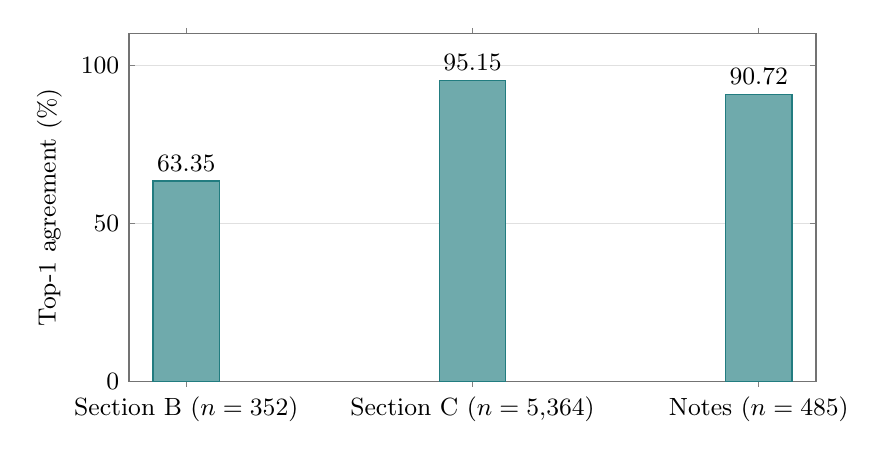
\begin{tikzpicture}
\begin{axis}[width=0.85\linewidth,height=6cm,ybar,bar width=24pt,
  ylabel={Top-1 agreement (\%)},ymin=0,ymax=110,
  symbolic x coords={B,C,Notes},xtick=data,
  xticklabels={Section B ($n=352$),Section C ($n=5{,}364$),Notes ($n=485$)},
  ymajorgrids=true,nodes near coords,nodes near coords style={font=\small},
  point meta=explicit symbolic]
\addplot[fill=teal!65,draw=teal] coordinates {(B,63.35) [63.35] (C,95.15) [95.15] (Notes,90.72) [90.72]};
\end{axis}
\end{tikzpicture}
\caption{Principle-label agreement by source. The bars compare explicitly tagged passages, concept-mapped passages, and principle notes using the filing-derived reference labels. Table~\ref{tab:source} gives confidence intervals calculated by resampling companies.}
\label{fig:source}
\end{figure}


\subsection{Recovered classifier performance and training history}
\label{sec:training_history}

The recovered seed-99 model matches 5,767 of 6,201 reference labels. Top-1 agreement is 93.00\% (95\% CI: 92.04--93.89\%). The reference label appears among the two highest predictions for 6,057 examples, giving 97.68\% Top-2 agreement (95\% CI: 97.10--98.21\%). Macro-F1 is 0.9158 (95\% CI: 0.9036--0.9277). The text-overlap check identifies 50 exact train/test matches across different companies, or 0.81\% of test rows. The supervised split has zero CIN overlap.

Figure~\ref{fig:training} shows the five recorded epochs for seed 99. Validation macro-F1 rises from 0.9048 at epoch 1 to 0.9194 at epoch 4, then reaches 0.9189 at epoch 5. Validation loss rises over the same period. F1 describes category decisions, while loss also considers prediction confidence. The recorded selection criterion chooses epoch 4 by validation macro-F1.

\begin{figure}[tbp]
\centering
\begin{subfigure}{0.48\linewidth}
\centering
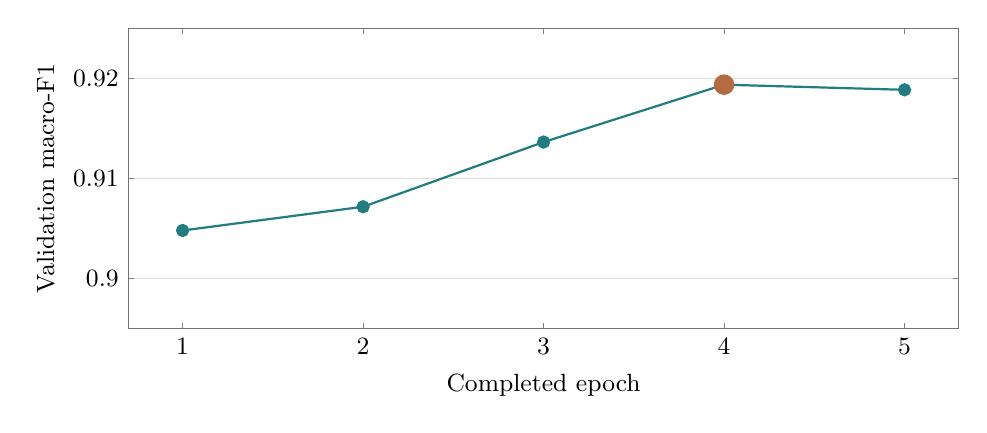
\begin{tikzpicture}
\begin{axis}[width=\linewidth,height=5.4cm,xlabel={Completed epoch},ylabel={Validation macro-F1},
  xmin=0.7,xmax=5.3,ymin=0.895,ymax=0.925,xtick={1,2,3,4,5},ymajorgrids=true,
  scaled y ticks=false,yticklabel style={/pgf/number format/fixed,/pgf/number format/precision=3}]
\addplot[teal,thick,mark=*] coordinates {(1,0.904818)(2,0.907187)(3,0.913640)(4,0.919368)(5,0.918854)};
\addplot[warm,only marks,mark=*,mark size=3.5pt] coordinates {(4,0.919368)};
\end{axis}
\end{tikzpicture}
\caption{Category agreement is highest at epoch 4.}
\end{subfigure}\hfill
\begin{subfigure}{0.48\linewidth}
\centering
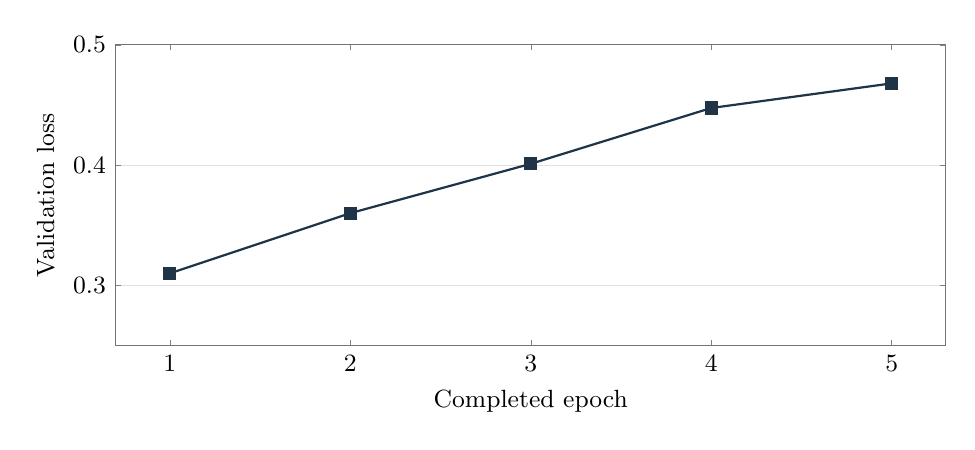
\begin{tikzpicture}
\begin{axis}[width=\linewidth,height=5.4cm,xlabel={Completed epoch},ylabel={Validation loss},
  xmin=0.7,xmax=5.3,ymin=0.25,ymax=0.50,xtick={1,2,3,4,5},ymajorgrids=true]
\addplot[ink,thick,mark=square*] coordinates {(1,0.310062)(2,0.360093)(3,0.401145)(4,0.447556)(5,0.468024)};
\end{axis}
\end{tikzpicture}
\caption{Loss records changes in prediction confidence.}
\end{subfigure}
\caption{Five recorded training epochs for seed 99. The marked point identifies checkpoint 7,460, selected by validation macro-F1. The two panels present category agreement and probability-based loss, showing the recorded basis for checkpoint selection.}
\label{fig:training}
\end{figure}


Table~\ref{tab:per_principle} groups performance by principle; Table~\ref{tab:source} groups performance by label source. Each principle row shows prediction reliability, reference-category coverage, and the balance between both. P7 has only 69 test examples, so the P7 estimate needs extra care. Figure~\ref{fig:per_principle} summarises F1, while the table also gives precision, recall, and example counts.

\begin{table}[tbp]
\centering\small
\caption{Results for nine principles on 6,201 text segments. Precision shows how often a predicted principle matches the reference. Recall shows how much of the reference category is found. F1 balances both.}
\label{tab:per_principle}
\begin{tabularx}{\linewidth}{@{}Yrrrr@{}}
\toprule\textbf{Principle} & \textbf{Support} & \textbf{Precision} & \textbf{Recall} & \textbf{F1}\\\midrule
P1: Ethics and governance & 773 & 0.9592 & 0.9431 & 0.9511 \\
P2: Sustainable goods and services & 808 & 0.9154 & 0.8837 & 0.8992 \\
P3: Employee and worker wellbeing & 1,715 & 0.9533 & 0.9644 & 0.9588 \\
P4: Stakeholder interests & 469 & 0.9611 & 0.9488 & 0.9549 \\
P5: Human rights & 449 & 0.9009 & 0.8508 & 0.8751 \\
P6: Environmental responsibility & 823 & 0.8943 & 0.9356 & 0.9145 \\
P7: Public policy advocacy & 69 & 0.8551 & 0.8551 & 0.8551 \\
P8: Inclusive growth & 368 & 0.8921 & 0.9212 & 0.9064 \\
P9: Consumer responsibility & 727 & 0.9259 & 0.9285 & 0.9272 \\
\midrule
Macro average & 6,201 & 0.9175 & 0.9146 & 0.9158\\\bottomrule
\end{tabularx}
\end{table}

\begin{figure}[tbp]
\centering
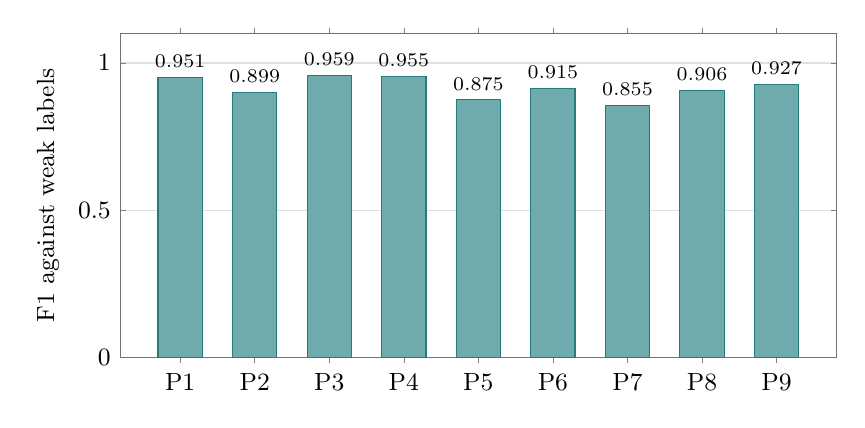
\begin{tikzpicture}
\begin{axis}[width=0.88\linewidth,height=5.7cm,ybar,bar width=16pt,ymin=0,ymax=1.10,
  ylabel={F1 against weak labels},symbolic x coords={P1,P2,P3,P4,P5,P6,P7,P8,P9},xtick=data,
  ymajorgrids=true,nodes near coords,nodes near coords style={font=\scriptsize,/pgf/number format/fixed,/pgf/number format/precision=3}]
\addplot[fill=teal!65,draw=teal] coordinates {(P1,0.9511)(P2,0.8992)(P3,0.9588)(P4,0.9549)(P5,0.8751)(P6,0.9145)(P7,0.8551)(P8,0.9064)(P9,0.9272)};
\end{axis}
\end{tikzpicture}
\caption{F1 by principle for the recovered classifier. A higher bar means a better balance of precision and recall against the recorded weak labels. P7 has 69 test examples, compared with 1,715 for P3. Table~\ref{tab:per_principle} gives all example counts and measures.}
\label{fig:per_principle}
\end{figure}


\subsection{Tests on excluded concepts and multiple labels}
\label{sec:concept_diagnostics}

Two kinds of separation are tested. The first, separating companies, asks whether the model can classify text segments from a company excluded from supervised training. The second, separating concepts, asks whether the model can classify text segments that answer reporting questions left out of labelled training. For the concept test, 17 Section C concepts were excluded, and 1,190 dataset rows were evaluated. On these same dataset rows, the full-concept model reaches 97.98\% Top-1 agreement, while the excluded-concept model reaches 87.31\%. The paired difference is $-10.67$ percentage points (95\% CI: $-12.36$ to $-8.96$). Before re-evaluation, both checkpoints passed strict parameter-name recovery.

The two models were not trained under identical conditions. The full-concept model uses seed 99. The excluded-concept model uses seed 42 and fewer training examples. The paired interval therefore describes the difference on shared test dataset rows under these conditions, and the gap reflects concept coverage, the number of training examples, and the seed together, not concept exclusion alone.

The excluded-concept training was repeated in three runs. The mean Top-1 agreement across the three runs is 81.64\%, with a sample standard deviation of 4.92 percentage points. The mean Top-2 agreement is 95.34\% (standard deviation 1.31 percentage points), and the mean macro-F1 is 0.6752 (standard deviation 0.0170). Figure~\ref{fig:concept} shows each run and the corresponding test size. The standard deviations measure how much the three runs differ from one another. All three runs reuse the original test-company group, and concept exclusion applies to labelled training only. The adaptation-corpus membership of the earlier model is described in Section~\ref{sec:classifier}.

\begin{figure}[tbp]
\centering
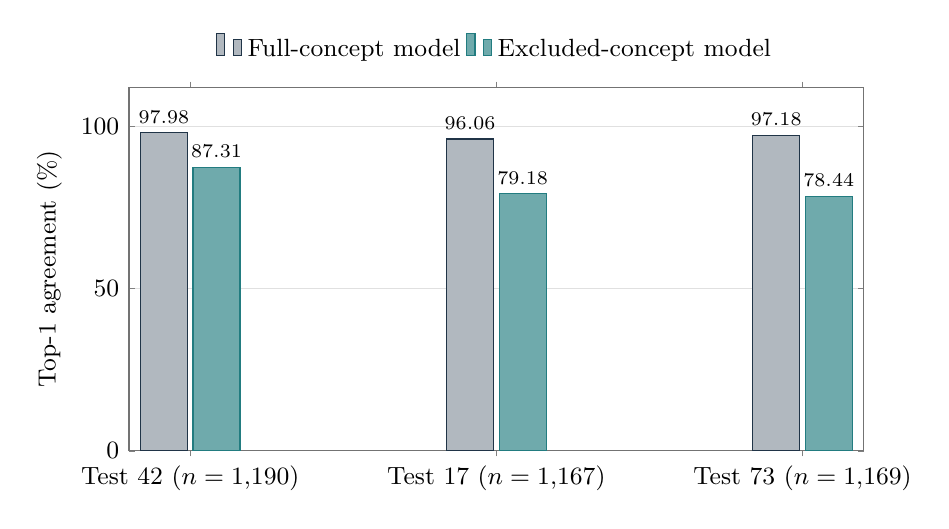
\begin{tikzpicture}
\begin{axis}[width=0.90\linewidth,height=6.2cm,ybar,bar width=17pt,ymin=0,ymax=112,
  ylabel={Top-1 agreement (\%)},symbolic x coords={H42,H17,H73},xtick=data,
  xticklabels={Test 42 ($n=1{,}190$),Test 17 ($n=1{,}167$),Test 73 ($n=1{,}169$)},
  ymajorgrids=true,legend style={at={(0.5,1.04)},anchor=south,legend columns=2},
  nodes near coords,nodes near coords style={font=\scriptsize,/pgf/number format/fixed,/pgf/number format/precision=2}]
\addplot[fill=ink!35,draw=ink] coordinates {(H42,97.98)(H17,96.06)(H73,97.18)};
\addlegendentry{Full-concept model}
\addplot[fill=teal!65,draw=teal] coordinates {(H42,87.31)(H17,79.18)(H73,78.44)};
\addlegendentry{Excluded-concept model}
\end{axis}
\end{tikzpicture}
\caption{Full-concept and excluded-concept training on three shared test groups. The tests contain 174, 173, and 174 companies from the original split. Excluded-concept mean agreement is 81.64\%, with sample standard deviation 4.92 percentage points across runs. Training examples and seeds are described in Section~\ref{sec:concept_diagnostics}; the standard deviation summarises variation across these runs.}
\label{fig:concept}
\end{figure}


\subsection{Frozen text-vagueness results}

Table~\ref{tab:detector} lists how the fixed detector performed on two separate groups of examples. The first group, Batches 1 and 2, has 80 earlier development examples. The reference label marks 37 text segments as vague, and the detector raises 41 flags. Only 29 of these flags agree with the reference. Out of 41 flags, 29 were right, which is a precision of 0.7073. Out of 37 vague examples, 29 were found, which is a recall of 0.7838. Accuracy counts every decision, flagged or not. Here 60 of the 80 decisions match the reference, so accuracy is 0.7500. F1, the balance between precision and recall, is 0.7436.

Batch 3 forms the second group. The 70 examples of this batch were labelled by AI, and not by the earlier development process. The detector flags 35 text segments, and 21 of the flags match the AI label. The AI label marks 26 text segments as vague, so the detector found 21 of 26. F1 for this group is 0.6885. Figure~\ref{fig:detector} puts precision, recall, and F1 of this group beside the 80-example group. The two groups differ in text segments and in the source of the reference, so the results are not merged.

\begin{table}[tbp]
\centering\small
\caption{Fixed text-vagueness detector on two label groups. The first row uses 80 development examples, and the second uses 70 AI-labelled examples. Reference conditions are stated in the evaluation text.}
\label{tab:detector}
\begin{tabularx}{\linewidth}{@{}Yrrrrr@{}}
\toprule\textbf{Reference labels} & \textbf{N} & \textbf{Accuracy} & \textbf{Precision} & \textbf{Recall} & \textbf{F1}\\\midrule
Historical development labels & 80 & 0.7500 & 0.7073 & 0.7838 & 0.7436\\
AI annotations & 70 & 0.7286 & 0.6000 & 0.8077 & 0.6885\\\bottomrule
\end{tabularx}
\end{table}

\begin{figure}[tbp]
\centering
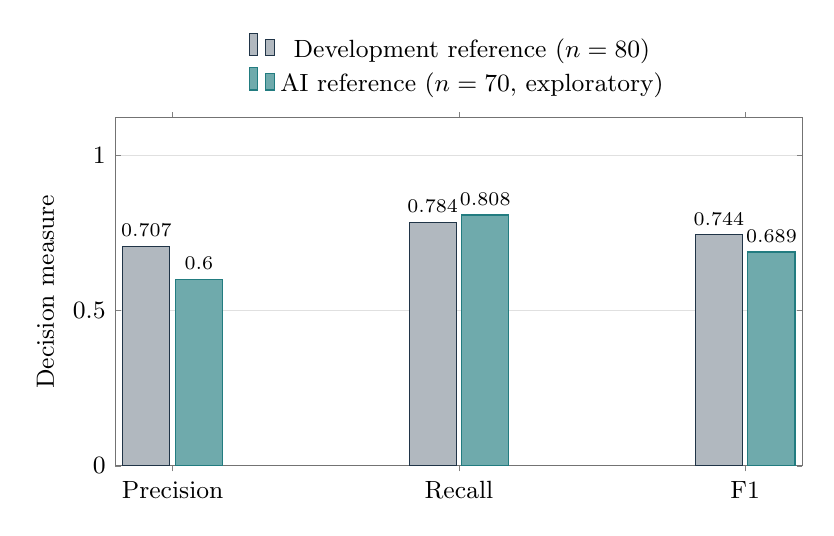
\begin{tikzpicture}
\begin{axis}[width=0.85\linewidth,height=6cm,ybar,bar width=17pt,ymin=0,ymax=1.12,
  ylabel={Decision measure},symbolic x coords={Precision,Recall,F1},xtick=data,
  ymajorgrids=true,legend style={at={(0.5,1.03)},anchor=south,legend columns=1},
  nodes near coords,nodes near coords style={font=\scriptsize,/pgf/number format/fixed,/pgf/number format/precision=3}]
\addplot[fill=ink!35,draw=ink] coordinates {(Precision,0.7073)(Recall,0.7838)(F1,0.7436)};
\addlegendentry{Development reference ($n=80$)}
\addplot[fill=teal!65,draw=teal] coordinates {(Precision,0.6000)(Recall,0.8077)(F1,0.6885)};
\addlegendentry{AI reference ($n=70$, exploratory)}
\end{axis}
\end{tikzpicture}
\caption{Precision, recall, and F1 for the fixed language detector. The first group contains 80 development examples; the second contains 70 AI-labelled examples. Precision describes how often a flag matches the reference, recall describes how many reference-vague passages are found, and F1 balances both. These measures cover the language branch.}
\label{fig:detector}
\end{figure}


\subsection{Supervised transfer versus zero-shot mapping}
\label{sec:eval_mapping}

The same 6,201 test text segments were ranked by two methods. The first is the MPNet definition-plus-anchor method, which has no training on the labelled data. The method reaches a Top-1 agreement of 67.63\% and a Top-2 agreement of 83.34\%. The second is the recovered supervised classifier, which was trained on the labels and reaches 93.00\% and 97.68\%. The confidence intervals for both methods are given in Table~\ref{tab:mapping}. The paired Top-1 difference shows the supervised classifier agreeing with the recorded principle label more often, by $+25.37$ percentage points (95\% CI: $+24.02$ to $+26.71$). The size of this gap should be read with care. Two things differ between the methods, the model representation and the access to labelled training, so the gap cannot be credited to the representation alone. Both results measure agreement with the recorded principle label.

\begin{table}[tbp]
\centering\small
\caption{Principle mapping on the same company-separated test rows. Intervals resample companies. The supervised row reuses the classifier result and is not a second independent test.}
\label{tab:mapping}
\begin{tabularx}{\linewidth}{@{}Yrrl@{}}
\toprule\textbf{Method} & \textbf{Top-1} & \textbf{Top-2} & \textbf{Macro-F1}\\\midrule
MPNet zero-shot hybrid & 67.63\% & 83.34\% & 0.6405\\
\quad 95\% interval & 66.45--68.93\% & 82.31--84.38\% & 0.6248--0.6567\\
Recovered supervised transfer & 93.00\% & 97.68\% & 0.9158\\
\quad 95\% interval & 92.04--93.89\% & 97.10--98.21\% & 0.9036--0.9277\\\bottomrule
\end{tabularx}
\end{table}

The supervised row reuses the classifier evaluation from the same company-separated test set. Both methods are compared against the filing-derived reference labels defined in Section~\ref{sec:labels}. The result is reported once as an underlying model evaluation and reused for the mapping application.

\subsection{Transparency Score compared with historical human ratings}

The historical human-rating group contains 20 companies. Pearson correlation measures how automated and human scores vary together: $r=0.6314$ (95\% CI: 0.2683--0.8519; $p=0.0028$). Spearman correlation compares score ranks: $\rho=0.6285$ (95\% CI: 0.2321--0.8540). Mean absolute error is 12.16 points, and root mean squared error, which gives larger errors more weight, is 15.19 points. The audit reports $r^2=0.3986$. This squared correlation describes association; no separate predictive regression was fitted for this result.

The historical comparison uses 20 company ratings from one documented source. The saved file contains both ratings and automated scores; rater blinding is not documented. The original Zensar text packet includes a URL-related extraction issue, and Geojit's business model differs from manufacturing-oriented reporting items. Both companies remain in the full group. The analysis uses the original ratings and fixed score formula, with all 20 cases retained; synthetic ratings and AI assessments are kept separate.

\subsection{Checking the API connection}

The audit records a successful principle-mapping API request for 360 ONE WAM LIMITED on 19 October 2026. The response identifies the recovered seed-99 classifier and checkpoint path. The returned 89.17\% summary is the average model probability for that filing. This request verifies model loading for one company.

\FloatBarrier
\section{Results Across Four Reporting Levels}
\label{sec:results}

The previous section tested the analysis methods. This section shows what the saved outputs look like in practice, so that an analyst can see how a single number is built and how the number compares with others. The outputs are presented at four levels: one company, selected companies in one sector, the full financial-sector group, and all recorded sectors. All company values come from the saved exports. A \emph{sector} is a group of companies with similar business activity, based on the recorded industry code. The examples connect the analysis of text segments with company scores and sector summaries.

The input for this section is the saved database of reports. The database contains 1,164 company records and 1,172 reports. The count of reports is higher because some companies filed reports for two years. The score export keeps one row for each of the 1,164 unique CINs and uses the most recent available report of each company, as selected by the script. These counts define the company collection used in all examples below.

\subsection{One company: from filed facts to an interpretable outcome}
\label{sec:case}

Triveni Turbine Limited serves as the worked example, since all four score components and a sector comparison are available for the company. The linked report ends on 31 March 2026 and contains 1,862 raw facts. Table~\ref{tab:case_facts} lists three figures, each with a value for the previous year and a value for the current year. For every figure, the concept, the unit, and the period are the same in both years, so the two values can be compared directly. Scope 1 emissions rise, while Scope 2 emissions and water withdrawal fall. The unit tCO2e stands for tonnes of carbon dioxide equivalent. Suppose a sentence claims that environmental performance improved. Scope 2 emissions and water withdrawal would support the sentence, but Scope 1 emissions would not. A general claim of improvement therefore has to be checked against each figure separately.

\begin{table}[tbp]
\centering\small
\caption{Filed values for Triveni Turbine, copied from report record 197 without correction. Concept, period, and unit links allow the pairs to be checked. The source links identify the original company values.}
\label{tab:case_facts}
\begin{tabularx}{\linewidth}{@{}Yrrl@{}}
\toprule\textbf{Filed measure} & \textbf{FY2024--25} & \textbf{FY2025--26} & \textbf{Filed unit}\\\midrule
Scope 1 emissions & 4,142.84 & 5,177.03 & tCO2e\\
Scope 2 emissions & 3,353.61 & 3,169.15 & tCO2e\\
Total water withdrawal & 88,662.28 & 85,611.54 & Kilolitres\\\bottomrule
\end{tabularx}
\end{table}

Each eligible text segment of the report receives a principle label from an explicit tag, a concept map, or a principle note. The classifier then ranks the nine principles, and the language detector marks evidence and vague wording. Every part of the saved score can be traced back to counts. The report has 613 accepted concepts out of the 1,057 concepts in the database, so Completeness is $100(613/1057)=57.99\%$. Scoring retains 52 concept--text pairs. Specificity of 63.46\% means that 33 of these 52 text segments contain a recognised evidence pattern. Clarity of 98.08\% means that one text segment is flagged as vague and 51 are not flagged. SDG breadth of 70.59\% means that 12 of the 17 goals are linked under the fixed map. Table~\ref{tab:case_score} applies the fixed weights to these four component percentages.

\begin{table}[tbp]
\centering\small
\caption{Transparency Score calculation for Triveni Turbine. Each percentage is multiplied by the weight. The final column shows the contribution before rounding the total.}
\label{tab:case_score}
\begin{tabularx}{\linewidth}{@{}Yrrr@{}}
\toprule\textbf{Component} & \textbf{Percentage} & \textbf{Weight} & \textbf{Contribution}\\\midrule
Completeness & 57.99 & 0.40 & 23.196\\
Specificity & 63.46 & 0.30 & 19.038\\
Clarity & 98.08 & 0.20 & 19.616\\
SDG breadth & 70.59 & 0.10 & 7.059\\\midrule
\textbf{Transparency Score} & & & \textbf{68.91}\\\bottomrule
\end{tabularx}
\end{table}

Equation~\eqref{eq:ts} gives $23.196+19.038+19.616+7.059=68.909$, which is rounded to 68.91. Figure~\ref{fig:company_contributions} plots each weighted contribution. The company belongs to the Machinery and Equipment group, which contains 36 companies with a mean score of 49.46. The \emph{percentile} of a company is the percentage of companies in the same sector with a strictly lower score. Triveni Turbine has a percentile of 94.4, which places the report near the upper end of this peer group.

\begin{figure}[tbp]
\centering
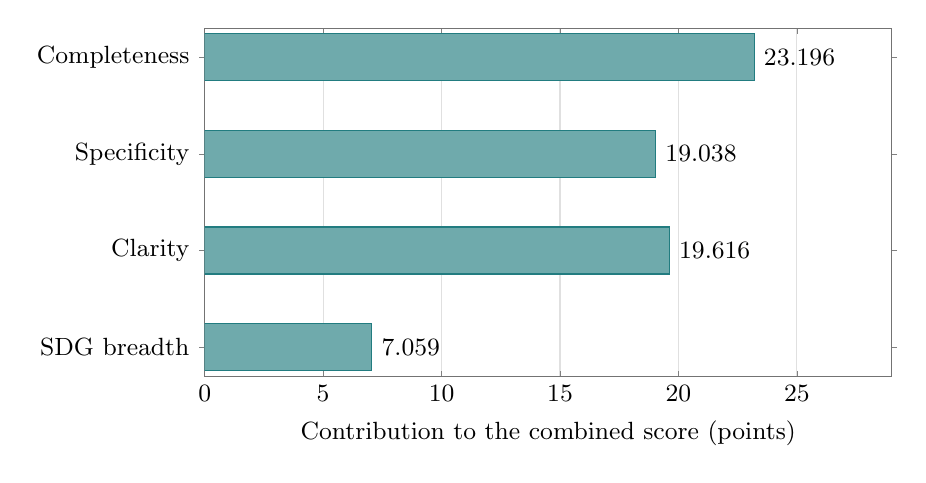
\begin{tikzpicture}
\begin{axis}[width=0.85\linewidth,height=6cm,xbar,bar width=17pt,
  xlabel={Contribution to the combined score (points)},xmin=0,xmax=29,
  symbolic y coords={SDG breadth,Clarity,Specificity,Completeness},ytick=data,xmajorgrids=true,
  nodes near coords,nodes near coords style={font=\small,/pgf/number format/fixed,/pgf/number format/precision=3}]
\addplot[fill=teal!65,draw=teal] coordinates {(7.059,SDG breadth)(19.616,Clarity)(19.038,Specificity)(23.196,Completeness)};
\end{axis}
\end{tikzpicture}
\caption{How the Triveni Turbine score is calculated. Each bar is the component percentage multiplied by the fixed weight. Completeness adds 23.196 points, Specificity 19.038, Clarity 19.616, and SDG breadth 7.059. The total is 68.909, rounded to 68.91. The bars show each component's contribution to the combined score.}
\label{fig:company_contributions}
\end{figure}

\FloatBarrier

\subsection{Selected financial companies: component differences and available years}
\label{sec:selected_finance}

The second level compares companies inside one sector. The saved \emph{Financial Services (excl. Insurance)} group has 94 companies. Table~\ref{tab:financial_selected} shows the four highest and the three lowest scores. These companies show the range of scores and are not a random sample. The next subsection summarises the full group.

\begin{table}[tbp]
\centering\small
\caption{Financial-company examples from the high and low ends of the score range. FY end 2026 and 2025 mean 31 March of those years. $C$, $Sp$, $Cl$, and $G$ are percentages; TS is the combined score. Years were reconstructed from the latest report of each CIN.}
\label{tab:financial_selected}
\begin{tabularx}{\linewidth}{@{}Yrrrrrr@{}}
\toprule\textbf{Company} & \textbf{FY end} & \textbf{$C$} & \textbf{$Sp$} & \textbf{$Cl$} & \textbf{$G$} & \textbf{TS}\\\midrule
REC & 2026 & 56.01 & 57.69 & 98.08 & 82.35 & 67.56 \\
Mahindra \& Mahindra Financial Services & 2026 & 67.83 & 49.15 & 98.31 & 29.41 & 64.48 \\
YES BANK & 2026 & 60.45 & 46.67 & 92.00 & 70.59 & 63.64 \\
KOTAK MAHINDRA BANK & 2026 & 61.21 & 59.42 & 95.65 & 17.65 & 63.21 \\
Fedbank Financial Services & 2025 & 31.98 & 12.12 & 75.76 & 0.00 & 31.58 \\
Nalwa Sons Investments & 2025 & 31.13 & 10.26 & 74.36 & 0.00 & 30.40 \\
Vardhman Holdings & 2025 & 35.00 & 2.78 & 75.00 & 0.00 & 29.83 \\
\bottomrule
\end{tabularx}
\end{table}

REC Limited scores 67.56, and Vardhman Holdings scores 29.83. Specificity is 57.69\% for REC and 2.78\% for Vardhman Holdings, and Completeness is 56.01\% and 35.00\%. Because both scores use the same formula, the component view shows exactly where the two disclosures differ. An analyst should also consider the business model, the recorded sector, the applicable reporting items, and the report year before drawing a conclusion from such a comparison.

A year-wise comparison needs two reports from the same company. For ESAF Small Finance Bank, Completeness rises from 34.34\% to 54.59\%, Specificity from 30.23\% to 41.30\%, and Clarity from 93.02\% to 93.48\%. SDG breadth stays at 11.76\%. The combined score rises from 42.59 to 54.10, which is a gain of 11.51 points. Completeness contributes about 8.10 points, Specificity 3.32 points, and Clarity 0.09 points. This breakdown links each component change to the change in the combined score.

Table~\ref{tab:esaf} shows all eight companies that have reports for two years. Six scores rise and two fall. The group mean rises from 45.17 to 50.40, a change of 5.23 points. The last column names the component with the largest absolute weighted contribution to each change, and the other components make up the remaining difference. Supplementary Table~\ref{tab:supp_paired} keeps both report records, the year labels, and every component for the eight companies.

\begin{table}[tbp]
\centering\small
\caption{Two-year Transparency Scores for all eight available companies. Changes and weighted contributions are score points. $C$, $Sp$, $Cl$, and $G$ are defined in Eq.~\eqref{eq:ts}. The last column gives the component with the largest absolute contribution to the change.}
\label{tab:esaf}
\begin{tabularx}{\linewidth}{@{}Yrrrr@{}}
\toprule\textbf{Company} & \textbf{FY2024--25} & \textbf{FY2025--26} & \textbf{Change} & \textbf{Largest contribution}\\\midrule
Praj Industries & 38.55 & 50.30 & +11.75 & $C$: +9.91 \\
ESAF Small Finance Bank & 42.59 & 54.10 & +11.51 & $C$: +8.10 \\
Sudarshan Colorants & 49.74 & 58.78 & +9.04 & $Sp$: +7.00 \\
Gopal Snacks & 41.30 & 47.29 & +5.99 & $Sp$: +8.53 \\
G R Infraprojects & 35.94 & 38.87 & +2.93 & $Sp$: +3.07 \\
Sudarshan Chemical & 62.95 & 65.32 & +2.37 & $G$: +2.35 \\
VIP Industries & 45.91 & 45.56 & -0.35 & $Cl$: -2.36 \\
SML Mahindra & 44.38 & 42.98 & -1.40 & $Cl$: -1.17 \\
\midrule
Group mean & 45.17 & 50.40 & +5.23 & \na\\\bottomrule
\end{tabularx}
\end{table}

\subsection{The complete financial-sector group}
\label{sec:all_finance}

The third level uses all 94 companies of the financial-sector group. The mean score is 48.17, the median is 49.79, and the standard deviation is 9.88. The \emph{median} is the middle score when all scores are sorted, and the \emph{standard deviation} shows how widely the scores are spread around the mean. Scores range from 29.83 to 67.56, a spread of 37.73 points. Mean Completeness is 49.77\%, Specificity 28.35\%, Clarity 90.67\%, and SDG breadth 16.27\%. Clarity is much higher than Specificity. This gap shows that avoiding vague phrases is not the same as giving concrete evidence.

The latest report of each company ends in March 2026 for 77 companies and in March 2025 for 17 companies. The year labels were reconstructed for each CIN from the database using the latest-report rule of the script, because the original score CSV does not contain a report identifier. The group is therefore a collection of the latest available reports. The separate eight-company comparison above uses two reports per company to show year-wise changes.

\begin{table}[tbp]
\begin{singlepagetable}
\centering\small
\caption{All 94 financial companies grouped by score. Each company appears in one band. Component columns give mean percentages; TS gives the mean combined score. Supplementary Table~\ref{tab:supp_financial} lists every company, reconstructed report year, and sector percentile.}
\label{tab:all_financial}
\begin{tabularx}{\linewidth}{@{}Yrrrrrrr@{}}
\toprule\textbf{Score band} & \textbf{N} & \textbf{Mean TS} & \textbf{Range} & \textbf{$C$} & \textbf{$Sp$} & \textbf{$Cl$} & \textbf{$G$}\\\midrule
60.00--69.99 & 11 & 62.39 & 60.01--67.56 & 61.17 & 47.24 & 95.25 & 47.06 \\
50.00--59.99 & 35 & 54.77 & 50.23--59.84 & 60.69 & 32.94 & 94.07 & 17.98 \\
40.00--49.99 & 26 & 45.22 & 40.57--49.96 & 45.85 & 26.05 & 89.79 & 11.08 \\
Below 40.00 & 22 & 34.05 & 29.83--39.80 & 31.33 & 14.30 & 84.02 & 4.28 \\
\midrule
All financial companies & 94 & 48.17 & 29.83--67.56 & 49.77 & 28.35 & 90.67 & 16.27\\\bottomrule
\end{tabularx}
\end{singlepagetable}
\end{table}

Table~\ref{tab:all_financial} groups the scores into four bands. Eleven companies score at least 60, 35 companies score from 50 to below 60, 26 companies score from 40 to below 50, and 22 companies score below 40. Mean Specificity is 14.30\% in the lowest band and 47.24\% in the highest band. The bands therefore show both the spread of the combined score and the component values behind each band.

The financial-sector mean is 0.56 points below the overall mean of 48.73 for all companies. This places the sector close to the full company collection, while the company rows show how much the scores vary inside the sector.

\FloatBarrier
\subsection{All sectors: coverage, score distribution, and interpretation}
\label{sec:all_sectors}

The final level covers 1,164 company scores across 72 recorded sectors. Scores range from 26.88 to 75.58, with a mean of 48.73 and a median of 47.25. Forty-seven sectors contain at least five companies and account for 1,109 scores. The other 25 sectors contain 55 companies in total. Table~\ref{tab:all_sectors} lists the 47 larger sectors separately and combines the smaller sectors in one labelled row. Supplementary Table~\ref{tab:supp_sectors} lists all 72 sectors.

Among the 47 sectors used for comparison, Warehousing and Transport Support has the highest mean, 54.55 across six companies. Wearing Apparel has the lowest mean, 42.33 across six companies, and Education follows at 42.43, also across six companies. The highest and lowest means differ by 12.22 points. These are descriptive comparisons of the saved company scores, and the number of companies is shown beside each mean because small sectors can change easily with one company.

The larger sectors give more stable context. Chemicals Manufacturing has 101 companies with a mean of 49.56, Financial Services has 94 companies with a mean of 48.17, and Pharmaceuticals has 65 companies with a mean of 51.18. The scores of Pharmaceuticals range from 32.38 to 73.72, and the scores of Chemicals Manufacturing range from 32.18 to 75.34. Reporting both the sector mean and the company range shows the differences inside each recorded sector, not only between sectors.

\begin{table}[p]
\begin{singlepagetable}
\centering
\begingroup
\footnotesize
\setlength{\tabcolsep}{5pt}
\renewcommand{\arraystretch}{1.00}
\caption{Sector scores for all 1,164 companies. The 47 sectors with at least five companies are listed separately. The other 25 sectors are combined below the line. SD shows the spread of company scores. The main comparison uses a five-company reporting threshold. Supplementary Table~\ref{tab:supp_sectors} lists all 72 sectors and medians.}
\label{tab:all_sectors}
\begin{tabularx}{\linewidth}{@{}Yrrrr@{}}
\toprule\textbf{Sector or reporting group} & \textbf{N} & \textbf{Mean TS} & \textbf{Range} & \textbf{SD}\\\midrule
Chemicals Manufacturing & 101 & 49.56 & 32.18--75.34 & 9.32 \\
Financial Services (excl. Insurance) & 94 & 48.17 & 29.83--67.56 & 9.88 \\
Pharmaceuticals & 65 & 51.18 & 32.38--73.72 & 10.06 \\
Basic Metals & 60 & 50.80 & 34.61--75.58 & 10.87 \\
Electrical Equipment & 51 & 48.80 & 26.88--67.03 & 9.56 \\
Computer Programming and Information Technology Services & 49 & 50.24 & 32.89--73.98 & 12.25 \\
Non-Metallic Mineral Products & 40 & 50.36 & 35.66--69.20 & 8.69 \\
Food Products Manufacturing & 38 & 47.57 & 30.04--69.86 & 9.60 \\
Motor Vehicles & 37 & 51.76 & 33.29--70.12 & 9.98 \\
Machinery and Equipment & 36 & 49.46 & 35.61--69.67 & 10.06 \\
Rubber and Plastics & 36 & 49.22 & 35.44--73.87 & 9.90 \\
Auxiliary Financial Services & 31 & 47.26 & 27.67--61.39 & 9.08 \\
Electricity, Gas, Steam and AC Supply & 31 & 53.67 & 31.95--74.23 & 11.49 \\
Fabricated Metal Products & 27 & 50.29 & 35.03--65.72 & 8.66 \\
Textiles & 26 & 47.44 & 31.77--67.65 & 10.16 \\
Wholesale Trade & 24 & 45.46 & 28.05--64.86 & 12.39 \\
Civil Engineering & 23 & 48.31 & 31.99--66.15 & 10.84 \\
Retail Trade & 21 & 43.06 & 34.22--56.45 & 6.12 \\
Construction & 20 & 48.73 & 36.58--63.25 & 8.32 \\
Insurance and Pension Funding & 20 & 51.52 & 29.92--64.17 & 10.12 \\
Real Estate Activities & 19 & 47.90 & 35.17--63.42 & 8.78 \\
Human Health Activities & 18 & 46.37 & 33.92--62.86 & 8.12 \\
Information Service Activities & 18 & 47.39 & 33.97--64.19 & 9.71 \\
Computer, Electronic and Optical Products & 17 & 47.46 & 32.93--65.45 & 7.59 \\
Other Transport Equipment & 17 & 50.83 & 37.67--66.89 & 9.39 \\
Other Manufacturing & 16 & 46.11 & 30.59--63.81 & 10.19 \\
Telecommunications & 15 & 50.63 & 36.57--69.19 & 11.43 \\
Accommodation & 14 & 48.67 & 31.28--67.57 & 10.06 \\
Mining and Quarrying & 13 & 47.40 & 29.01--73.16 & 13.27 \\
Beverages Manufacturing & 10 & 47.30 & 34.70--67.71 & 13.18 \\
Other (Division 99) & 10 & 48.39 & 34.80--73.44 & 12.12 \\
Wholesale/Retail Trade - Motor Vehicles & 10 & 49.25 & 37.40--67.92 & 11.47 \\
Architecture and Engineering & 9 & 48.50 & 37.49--64.86 & 10.06 \\
Coke and Refined Petroleum & 9 & 52.32 & 38.20--69.63 & 11.13 \\
Paper Products & 9 & 43.27 & 33.42--48.93 & 4.88 \\
Broadcasting & 8 & 43.65 & 31.66--52.74 & 7.64 \\
Land Transport & 7 & 47.42 & 34.72--63.63 & 10.11 \\
Water Supply and Waste Management & 7 & 43.33 & 36.73--56.76 & 8.29 \\
Wood Products & 7 & 46.18 & 36.16--64.51 & 9.72 \\
Education & 6 & 42.43 & 33.28--55.70 & 7.74 \\
Furniture & 6 & 51.28 & 36.17--65.29 & 9.25 \\
Other Professional/Technical Activities & 6 & 48.43 & 38.73--57.90 & 8.70 \\
Scientific R\&D & 6 & 44.90 & 38.95--52.11 & 5.71 \\
Warehousing and Transport Support & 6 & 54.55 & 37.82--67.03 & 10.34 \\
Wearing Apparel & 6 & 42.33 & 37.17--48.78 & 4.50 \\
Leather Products & 5 & 50.00 & 42.14--58.86 & 7.80 \\
Water Transport & 5 & 48.37 & 38.70--61.22 & 9.75 \\
\midrule
Other 25 small sectors (combined) & 55 & 44.08 & 27.56--70.97 & 8.95\\
\textbf{All 72 sectors} & \textbf{1,164} & \textbf{48.73} & \textbf{26.88--75.58} & \textbf{9.98}\\\bottomrule
\end{tabularx}
\endgroup
\end{singlepagetable}
\end{table}
\FloatBarrier

The Pharmaceuticals sector gives a closer view of the differences inside one sector. Dabur India scores 73.72 and Kopran scores 32.38, a gap of 41.34 points. Completeness is 73.13\% for Dabur India and 32.92\% for Kopran, and Specificity is 57.38\% and 23.68\%. Clarity exceeds 85\% for 58 of the 65 companies, so the gap between companies comes mainly from Completeness and Specificity. Supplementary Table~\ref{tab:supp_pharma} keeps the four highest and three lowest examples with every component.

The four levels allow an analyst to move from a component calculation to a company score, then to a sector comparison, and finally to the full company collection. At each step, the denominator, the source records, and the meaning of the output remain visible. This structure supports both detailed review of one report and summary comparison across many reports.

\FloatBarrier
\section{Conclusion}
\label{sec:conclusion}

Reviewing a BRSR report means following a claim to the evidence behind the claim, and then to a summary for the whole company. GRASP supports this in one workflow. Each report is stored in a structured form, and the principle labels come from the structure of the report and not from a person reading the text. A classifier sorts text segments into the nine principles, a detector flags vague wording, and numerical checks create review records. A four-part Transparency Score then summarises each company. Text segments and facts remain tied to the same report, so an analyst can always return to the source. The source of every label stays visible during evaluation, and every score component has an explicit formula. The vagueness detector built for the flagging step is used again to calculate Clarity, which carries a weight of 20\% in the score. The numerical review records stay outside the score as separate outputs.

The classifier was tested on 6,201 text segments from 175 companies that were not used for supervised training. Here, 6,201 is a count of text segments, and the test group does not contain 6,201 reports or 6,201 companies. For 93.00\% of these text segments, the classifier predicts the same principle as the weak label (95\% confidence interval: 92.04--93.89\%). A confidence interval is a range that is likely to contain the true value. The macro-F1 is 0.9158, which is the average F1 score over the nine principles, so a small principle counts as much as a large one. The result depends on where the label came from. Agreement is 63.35\% for explicitly tagged narratives, 95.15\% for concept-mapped narratives, and 90.72\% for principle notes. A weak label is taken from the structure of the report, so each of these values measures agreement with the recorded assignment. None of these agreement values is an independent judgement of what the text means.

The other outputs were tested separately. On 80 development examples, the fixed vagueness detector reaches an F1 score of 0.7436. The Transparency Score was compared with 20 historical human ratings, and the Pearson correlation is $r=0.6314$ (95\% confidence interval: 0.2683--0.8519). This correlation shows how closely two sets of scores rise and fall together. The conditions behind each result are described in Section~\ref{sec:evaluation}. Each reported result relates to the corresponding task: principle assignment, language screening, or score comparison.

The saved outputs cover 1,164 companies in 72 recorded sectors and are presented at four levels: one worked company, selected companies within a sector, the complete financial-sector group, and all sectors. Financial-sector scores range from 29.83 to 67.56. Among the 47 sectors with at least five companies, Wearing Apparel has the lowest mean score, 42.33, and Warehousing and Transport Support has the highest, 54.55. Eight companies have reports for two years, and the group mean score moved from 45.17 to 50.40, a gain of 5.23 points. Individually, six of the eight companies gained and two lost. For each company, the component breakdown names the part of the disclosure that drove the change. For example, Completeness explains most of the gain for ESAF Small Finance Bank, which rises by 11.51 points. Together, the company, sector, and year views allow an analyst to inspect the results both in detail and in summary.

This work can be extended using multiple levels. The first concerns the data. Collection can be widened to include annexures, charts, and additional annual reports. The second concerns the models. New comparisons need larger datasets with principle labels. Blind human-rating studies would also help, because reviewers would rate reports without seeing the automated scores. The language adaptation step can be repeated with text from declared training companies only, and then tested on newly collected companies. Business descriptions are a further source of information. A description of what a company does can make the sector assignment more detailed, and the same description can show which reporting items apply to the company. The numerical checks have room to grow as well. At present, an analyst compares the definition of the measure, the unit, the period, and the business boundary by hand. A future check could make these comparisons before a review record is created. More annual reports would also help. With several years available, the same companies can be compared again and again under one recorded score version. Finally, the report-based approach can be tested on international sustainability standards. For each standard, the reporting items must first be mapped one by one, and the results must then be evaluated separately.

\begin{thebibliography}{99}
\small

\bibitem{sebi2021}
Securities and Exchange Board of India, ``Business responsibility and sustainability reporting by listed entities,'' Circular SEBI/HO/CFD/CMD-2/P/CIR/2021/562, 10 May 2021. \url{https://www.sebi.gov.in/legal/circulars/may-2021/business-responsibility-and-sustainability-reporting-by-listed-entities_50096.html}.

\bibitem{webersinke2021}
N. Webersinke, M. Kraus, J. A. Bingler, and M. Leippold, ``ClimateBERT: A pretrained language model for climate-related text,'' arXiv:2110.12010, 2021. \url{https://arxiv.org/abs/2110.12010}.

\bibitem{ni2023}
J. Ni et al., ``CHATREPORT: Democratizing sustainability disclosure analysis through LLM-based tools,'' in \emph{Proceedings of EMNLP: System Demonstrations}, 2023, pp. 21--51. \url{https://doi.org/10.18653/v1/2023.emnlp-demo.3}.

\bibitem{zou2025}
Y. Zou et al., ``ESGReveal: An LLM-based approach for extracting structured data from ESG reports,'' \emph{Journal of Cleaner Production}, vol. 489, article 144572, 2025. \url{https://doi.org/10.1016/j.jclepro.2024.144572}.

\bibitem{calamai2025}
T. Calamai, O. Balalau, T. Le Guenedal, and F. M. Suchanek, ``Corporate greenwashing detection in text---a survey,'' arXiv:2502.07541, 2025. \url{https://arxiv.org/abs/2502.07541}.

\bibitem{garg2025}
A. Garg, K. Upadhyay, D. Arora, V. Avashia, J. Shah, and V. Gupta, \emph{Analysis and Insights from ESG Disclosures Submitted by 1012 Indian Businesses under BRSR Guidelines (2022--23)}. Indian Institute of Management Ahmedabad, NIIF Chair in ESG, 2025. \url{https://www.iima.ac.in/sites/default/files/2025-02/BRSR%20Report_2-12-2024.pdf}.

\bibitem{devlin2019}
J. Devlin, M.-W. Chang, K. Lee, and K. Toutanova, ``BERT: Pre-training of deep bidirectional transformers for language understanding,'' in \emph{Proceedings of NAACL-HLT}, 2019, pp. 4171--4186. \url{https://doi.org/10.18653/v1/N19-1423}.

\bibitem{gururangan2020}
S. Gururangan et al., ``Don't stop pretraining: Adapt language models to domains and tasks,'' in \emph{Proceedings of ACL}, 2020, pp. 8342--8360. \url{https://doi.org/10.18653/v1/2020.acl-main.740}.

\bibitem{reimers2019}
Nils Reimers and Iryna Gurevych, ``Sentence-BERT: Sentence embeddings using Siamese BERT-networks,'' in \emph{Proceedings of EMNLP-IJCNLP}, 2019, pp. 3982--3992. \url{https://doi.org/10.18653/v1/D19-1410}.

\bibitem{ratner2017}
A. Ratner, S. H. Bach, H. Ehrenberg, J. Fries, S. Wu, and C. R\'{e}, ``Snorkel: Rapid training data creation with weak supervision,'' \emph{Proceedings of the VLDB Endowment}, vol. 11, no. 3, pp. 269--282, 2017. \url{https://doi.org/10.14778/3157794.3157797}.

\bibitem{kapoor2023}
S. Kapoor and A. Narayanan, ``Leakage and the reproducibility crisis in machine-learning-based science,'' \emph{Patterns}, vol. 4, no. 9, article 100804, 2023. \url{https://doi.org/10.1016/j.patter.2023.100804}.

\bibitem{varini2020}
F. S. Varini, J. Boyd-Graber, M. Ciaramita, and M. Leippold, ``ClimaText: A dataset for climate change topic detection,'' arXiv:2012.00483, 2020. \url{https://arxiv.org/abs/2012.00483}.

\bibitem{bingler2022}
J. A. Bingler et al., ``Cheap talk and cherry-picking: What ClimateBERT has to say on corporate climate risk disclosures,'' \emph{Finance Research Letters}, vol. 47, article 102776, 2022. \url{https://doi.org/10.1016/j.frl.2022.102776}.

\bibitem{bingler2024}
J. A. Bingler, M. Kraus, M. Leippold, and N. Webersinke, ``How cheap talk in climate disclosures relates to climate initiatives, corporate emissions, and reputation risk,'' \emph{Journal of Banking \& Finance}, vol. 164, article 107191, 2024. \url{https://doi.org/10.1016/j.jbankfin.2024.107191}.

\bibitem{schimanski2023}
T. Schimanski, J. Bingler, M. Kraus, C. Hyslop, and M. Leippold, ``ClimateBERT-NetZero: Detecting and assessing net zero and reduction targets,'' in \emph{Proceedings of EMNLP}, 2023, pp. 15745--15756. \url{https://doi.org/10.18653/v1/2023.emnlp-main.975}.

\bibitem{vinella2024}
A. Vinella, M. Capetz, R. Pattichis, C. Chance, R. Ghosh, and K.-W. Chang, ``Leveraging language models to detect greenwashing,'' arXiv:2311.01469, revised 2024. \url{https://arxiv.org/abs/2311.01469}.

\bibitem{shankar2025}
R. Shankar and Q. Xu, ``Automated detection of greenwashing in Indian corporate sustainability reports using natural language processing,'' SSRN working paper 5294480, posted 2025; manuscript dated 30 June 2024. \url{https://doi.org/10.2139/ssrn.5294480}.

\bibitem{xbrl2013}
XBRL International, ``Extensible Business Reporting Language (XBRL) 2.1,'' Recommendation, corrected errata, 20 February 2013. \url{https://specifications.xbrl.org/work-product-index-group-base-spec-base-spec.html}.

\bibitem{song2020}
K. Song, X. Tan, T. Qin, J. Lu, and T.-Y. Liu, ``MPNet: Masked and permuted pre-training for language understanding,'' in \emph{Advances in Neural Information Processing Systems}, vol. 33, 2020, pp. 16857--16867. \url{https://arxiv.org/abs/2004.09297}.

\bibitem{un2015}
United Nations, ``The 17 goals,'' Sustainable Development Goals, 2030 Agenda, 2015. \url{https://sdgs.un.org/goals}.

\end{thebibliography}

\clearpage
\appendix
\section{Supplementary Tables}
\label{sec:supplementary}
\setcounter{table}{0}
\renewcommand{\thetable}{S\arabic{table}}
\renewcommand{\theHtable}{supp.\arabic{table}}

The following tables provide the complete records behind the compact company, sector, and year-wise results. Values are copied from the saved supplementary CSV files. No additional model training or inference is used. In all four tables, $C$ is Completeness, $Sp$ is Specificity, $Cl$ is Clarity, $G$ is SDG breadth, and TS is the Transparency Score. Component values are percentages. A sector percentile counts the share of companies in the same recorded sector with a strictly lower score.

\subsection{Complete financial-company results}

Table~\ref{tab:supp_financial} lists all 94 companies in the saved Financial Services (excl. Insurance) group. FY end gives the reporting end date reconstructed from the latest report recorded for each CIN. The original score export does not contain a report identifier; the date column follows the documented latest-report reconstruction. $N$ counts retained scoring text segments. Source: \artifact{table_S1_financial_companies.csv}.

{\footnotesize
\setlength{\tabcolsep}{3pt}
\renewcommand{\arraystretch}{1.12}
\begin{longtable}{@{}L{5.1cm}rrrrrrrr@{}}
\caption{Complete results for the 94 financial companies. Pctl. denotes the saved sector percentile; FY end is a reconstructed date.}\label{tab:supp_financial}\\
\toprule
\textbf{Company} & \textbf{FY end} & \textbf{$C$} & \textbf{$Sp$} & \textbf{$Cl$} & \textbf{$G$} & \textbf{TS} & \textbf{Pctl.} & \textbf{$N$}\\
\midrule\endfirsthead
\multicolumn{9}{l}{\textit{Table \thetable\ continued}}\\
\toprule
\textbf{Company} & \textbf{FY end} & \textbf{$C$} & \textbf{$Sp$} & \textbf{$Cl$} & \textbf{$G$} & \textbf{TS} & \textbf{Pctl.} & \textbf{$N$}\\
\midrule\endhead
\midrule\multicolumn{9}{r}{\textit{Continued on next page}}\\\endfoot
\bottomrule\endlastfoot
REC Limited & 2026-03-31 & 56.01 & 57.69 & 98.08 & 82.35 & 67.56 & 98.9 & 52 \\
Mahindra \& Mahindra Financial Services Limited & 2026-03-31 & 67.83 & 49.15 & 98.31 & 29.41 & 64.48 & 97.9 & 59 \\
YES BANK LIMITED & 2026-03-31 & 60.45 & 46.67 & 92.00 & 70.59 & 63.64 & 96.8 & 75 \\
KOTAK MAHINDRA BANK LIMITED & 2026-03-31 & 61.21 & 59.42 & 95.65 & 17.65 & 63.21 & 95.7 & 69 \\
ICICI Bank Limited & 2026-03-31 & 56.95 & 57.14 & 95.92 & 29.41 & 62.05 & 94.7 & 49 \\
PNB Housing Finance Limited & 2026-03-31 & 84.01 & 25.86 & 93.10 & 17.65 & 61.75 & 93.6 & 58 \\
KARUR VYSYA BANK LIMITED & 2026-03-31 & 54.78 & 45.10 & 100.00 & 58.82 & 61.32 & 92.6 & 51 \\
Punjab National Bank & 2026-03-31 & 54.21 & 42.11 & 92.98 & 82.35 & 61.15 & 91.5 & 57 \\
SBI Cards and Payment Services Limited & 2026-03-31 & 61.49 & 33.78 & 93.24 & 76.47 & 61.02 & 90.4 & 74 \\
IDFC FIRST Bank Limited & 2026-03-31 & 56.86 & 48.98 & 95.92 & 35.29 & 60.15 & 89.4 & 49 \\
Tata Capital Limited & 2026-03-31 & 59.04 & 53.70 & 92.59 & 17.65 & 60.01 & 88.3 & 54 \\
Axis Bank Limited & 2026-03-31 & 68.87 & 38.89 & 97.22 & 11.76 & 59.84 & 87.2 & 72 \\
Cholamandalam Financial Holdings Limited & 2026-03-31 & 67.74 & 25.76 & 95.45 & 58.82 & 59.80 & 86.2 & 66 \\
HDB Financial Services Limited & 2026-03-31 & 66.13 & 25.00 & 97.50 & 52.94 & 58.75 & 85.1 & 80 \\
State Bank of India (“SBI/the Bank/Bank”) & 2026-03-31 & 57.05 & 45.00 & 88.33 & 47.06 & 58.69 & 84.0 & 60 \\
Home First Finance Company India Limited & 2026-03-31 & 67.46 & 38.00 & 98.00 & 5.88 & 58.57 & 83.0 & 50 \\
THE KARNATAKA BANK LIMITED & 2025-03-31 & 63.67 & 41.18 & 96.08 & 11.76 & 58.21 & 81.9 & 51 \\
IndusInd Bank & 2026-03-31 & 68.78 & 28.81 & 94.92 & 29.41 & 58.08 & 80.9 & 59 \\
L\&T Finance Limited & 2026-03-31 & 59.79 & 44.44 & 98.15 & 11.76 & 58.05 & 79.8 & 54 \\
MUTHOOT FINANCE LIMITED & 2026-03-31 & 67.83 & 33.33 & 98.15 & 5.88 & 57.35 & 78.7 & 54 \\
THE FEDERAL BANK LIMITED & 2026-03-31 & 69.82 & 28.57 & 95.71 & 11.76 & 56.82 & 77.7 & 70 \\
Power Finance Corporation Limited (PFC) & 2026-03-31 & 68.78 & 34.04 & 89.36 & 11.76 & 56.77 & 76.6 & 47 \\
AU Small Finance Bank Limited & 2026-03-31 & 58.09 & 43.40 & 96.23 & 11.76 & 56.68 & 75.5 & 53 \\
IIFL Finance Limited & 2026-03-31 & 59.32 & 47.06 & 88.24 & 11.76 & 56.67 & 74.5 & 51 \\
Cholamandalam Investment and Finance Company Limited & 2026-03-31 & 66.23 & 26.92 & 90.38 & 35.29 & 56.17 & 73.4 & 52 \\
Bandhan Bank Limited & 2026-03-31 & 55.63 & 44.44 & 94.44 & 11.76 & 55.65 & 72.3 & 54 \\
Aadhar Housing Finance Limited & 2026-03-31 & 56.01 & 46.15 & 90.38 & 11.76 & 55.50 & 71.3 & 52 \\
Housing \& Urban Development Corporation Limited & 2026-03-31 & 56.10 & 31.43 & 91.43 & 47.06 & 54.86 & 70.2 & 70 \\
Union Bank of India & 2026-03-31 & 64.81 & 25.00 & 93.18 & 23.53 & 54.41 & 69.1 & 44 \\
Shriram Finance Limited (SFL) & 2026-03-31 & 55.72 & 41.82 & 89.09 & 11.76 & 53.83 & 68.1 & 55 \\
Manappuram Finance Limited & 2026-03-31 & 54.02 & 38.00 & 98.00 & 11.76 & 53.78 & 67.0 & 50 \\
360 ONE WAM LIMITED & 2026-03-31 & 68.68 & 27.16 & 90.12 & 0.00 & 53.64 & 66.0 & 81 \\
Aditya Birla Capital Limited & 2026-03-31 & 53.93 & 39.02 & 95.12 & 11.76 & 53.48 & 64.9 & 41 \\
CANARA BANK & 2026-03-31 & 52.98 & 38.46 & 96.15 & 11.76 & 53.14 & 63.8 & 52 \\
CITY UNION BANK LIMITED & 2026-03-31 & 50.90 & 27.45 & 98.04 & 47.06 & 52.91 & 62.8 & 51 \\
Aptus Value Housing Finance India Limited & 2026-03-31 & 65.94 & 19.15 & 97.87 & 11.76 & 52.87 & 61.7 & 47 \\
Aavas Financiers Limited & 2025-03-31 & 61.78 & 32.61 & 82.61 & 11.76 & 52.19 & 60.6 & 46 \\
INDIAN RAILWAY FINANCE CORPORATION LIMITED & 2026-03-31 & 57.62 & 26.23 & 96.72 & 17.65 & 52.03 & 59.6 & 61 \\
Westlife Foodworld Limited & 2026-03-31 & 54.30 & 34.09 & 100.00 & 0.00 & 51.95 & 58.5 & 44 \\
BANK OF INDIA & 2026-03-31 & 53.64 & 30.95 & 100.00 & 11.76 & 51.92 & 57.4 & 42 \\
Punjab \& Sind Bank & 2026-03-31 & 64.05 & 21.88 & 90.62 & 11.76 & 51.48 & 56.4 & 32 \\
IDBI Bank Limited & 2026-03-31 & 56.29 & 32.20 & 94.92 & 0.00 & 51.16 & 55.3 & 59 \\
BANK OF BARODA & 2026-03-31 & 55.82 & 18.33 & 96.67 & 35.29 & 50.69 & 54.3 & 60 \\
POONAWALLA FINCORP LIMITED & 2026-03-31 & 57.24 & 30.43 & 86.96 & 11.76 & 50.59 & 53.2 & 46 \\
UCO BANK & 2026-03-31 & 54.97 & 25.00 & 97.92 & 11.76 & 50.25 & 52.1 & 48 \\
ANAND RATHI WEALTH LIMITED & 2026-03-31 & 64.14 & 22.86 & 88.57 & 0.00 & 50.23 & 51.1 & 35 \\
Jio Financial Services Limited & 2026-03-31 & 56.10 & 32.69 & 82.69 & 11.76 & 49.96 & 50.0 & 52 \\
SUNDARAM FINANCE LIMITED & 2026-03-31 & 65.85 & 15.79 & 86.84 & 11.76 & 49.62 & 48.9 & 38 \\
BANK OF MAHARASHTRA & 2026-03-31 & 52.22 & 27.78 & 94.44 & 11.76 & 49.29 & 47.9 & 36 \\
GIC Housing Finance Limited & 2026-03-31 & 59.79 & 15.09 & 94.34 & 11.76 & 48.49 & 46.8 & 53 \\
NORTHERN ARC CAPITAL LIMITED & 2026-03-31 & 31.88 & 47.83 & 100.00 & 11.76 & 48.28 & 45.7 & 23 \\
Can Fin Homes Limited & 2026-03-31 & 36.33 & 43.14 & 94.12 & 17.65 & 48.06 & 44.7 & 51 \\
RBL Bank Limited & 2026-03-31 & 52.13 & 20.00 & 92.50 & 23.53 & 47.71 & 43.6 & 40 \\
FIVE-STAR BUSINESS FINANCE LIMITED & 2026-03-31 & 54.78 & 19.61 & 98.04 & 0.00 & 47.40 & 42.6 & 51 \\
Satin Creditcare Network Limited & 2026-03-31 & 37.37 & 38.78 & 95.92 & 11.76 & 46.94 & 41.5 & 49 \\
INDIAN OVERSEAS BANK & 2026-03-31 & 53.55 & 26.15 & 76.92 & 17.65 & 46.41 & 40.4 & 65 \\
Indian Bank & 2026-03-31 & 56.29 & 18.18 & 90.91 & 0.00 & 46.15 & 39.4 & 33 \\
UTKARSH SMALL FINANCE BANK LIMITED & 2026-03-31 & 34.53 & 43.59 & 87.18 & 11.76 & 45.50 & 38.3 & 39 \\
Muthoot Microfin Limited & 2026-03-31 & 35.76 & 29.09 & 94.55 & 35.29 & 45.47 & 37.2 & 55 \\
Capri Global Capital Limited & 2025-03-31 & 32.07 & 29.27 & 90.24 & 52.94 & 44.95 & 36.2 & 41 \\
Tata Investment Corporation Limited & 2026-03-31 & 59.41 & 15.22 & 76.09 & 11.76 & 44.72 & 35.1 & 46 \\
The South Indian Bank Limited & 2026-03-31 & 35.38 & 30.23 & 100.00 & 11.76 & 44.40 & 33.0 & 43 \\
Central Bank of India & 2026-03-31 & 51.18 & 17.86 & 92.86 & 0.00 & 44.40 & 33.0 & 28 \\
Fusion Finance Limited & 2026-03-31 & 36.61 & 32.69 & 96.15 & 0.00 & 43.68 & 31.9 & 52 \\
Spandana Sphoorty Financial Limited & 2026-03-31 & 33.49 & 45.71 & 80.00 & 0.00 & 43.11 & 30.9 & 35 \\
CSB BANK LIMITED & 2026-03-31 & 36.05 & 26.09 & 93.48 & 11.76 & 42.12 & 28.7 & 46 \\
JSW HOLDINGS LIMITED & 2026-03-31 & 66.89 & 2.44 & 73.17 & 0.00 & 42.12 & 28.7 & 41 \\
TVS Holdings Limited & 2026-03-31 & 54.78 & 10.00 & 86.00 & 0.00 & 42.11 & 27.7 & 50 \\
Sammaan Capital Limited & 2025-03-31 & 35.48 & 26.67 & 91.11 & 11.76 & 41.59 & 26.6 & 45 \\
Bajaj Holdings \& Investment Limited & 2026-03-31 & 55.72 & 8.00 & 84.00 & 0.00 & 41.49 & 25.5 & 25 \\
PNB Gilts Ltd. & 2025-03-31 & 37.37 & 29.27 & 87.80 & 0.00 & 41.29 & 24.5 & 41 \\
SBFC Finance Limited & 2026-03-31 & 31.22 & 26.19 & 95.24 & 11.76 & 40.57 & 23.4 & 42 \\
Vakrangee Limited & 2025-03-31 & 33.49 & 15.38 & 94.23 & 29.41 & 39.80 & 22.3 & 52 \\
IFCI Limited & 2025-03-31 & 33.30 & 19.61 & 86.27 & 29.41 & 39.40 & 21.3 & 51 \\
DCB Bank Limited & 2026-03-31 & 33.77 & 25.40 & 90.48 & 0.00 & 39.22 & 20.2 & 63 \\
EQUITAS SMALL FINANCE BANK LIMITED & 2026-03-31 & 34.15 & 18.18 & 87.88 & 0.00 & 36.69 & 19.1 & 33 \\
INDIA SHELTER FINANCE CORPORATION LIMITED & 2026-03-31 & 34.72 & 19.51 & 78.05 & 11.76 & 36.53 & 18.1 & 41 \\
Raymond Limited & 2026-03-31 & 31.98 & 21.43 & 78.57 & 11.76 & 36.11 & 17.0 & 42 \\
SURYODAY SMALL FINANCE BANK LIMITED & 2026-03-31 & 30.37 & 16.67 & 90.00 & 0.00 & 35.15 & 16.0 & 30 \\
SUMMIT SECURITIES LIMITED & 2026-03-31 & 24.98 & 13.51 & 94.59 & 11.76 & 34.14 & 14.9 & 37 \\
Arman Financial Services Limited & 2025-03-31 & 29.99 & 18.18 & 81.82 & 0.00 & 33.81 & 13.8 & 33 \\
Ugro Capital Limited & 2026-03-31 & 28.48 & 13.64 & 90.91 & 0.00 & 33.67 & 12.8 & 22 \\
IndoStar Capital Finance Limited & 2025-03-31 & 29.23 & 11.43 & 91.43 & 0.00 & 33.41 & 11.7 & 35 \\
SG Finserve Limited & 2026-03-31 & 29.52 & 15.79 & 84.21 & 0.00 & 33.39 & 10.6 & 19 \\
Dolat Algotech Limited & 2025-03-31 & 28.86 & 9.09 & 95.45 & 0.00 & 33.36 & 9.6 & 22 \\
Religare Enterprises Limited & 2025-03-31 & 38.98 & 6.00 & 78.00 & 0.00 & 32.99 & 8.5 & 50 \\
MAS FINANCIAL SERVICES LIMITED & 2026-03-31 & 35.29 & 10.20 & 77.55 & 0.00 & 32.69 & 7.4 & 49 \\
Nahar Capital and Financial Services Limited & 2025-03-31 & 27.53 & 10.81 & 89.19 & 0.00 & 32.09 & 6.4 & 37 \\
Dhani Services Limited & 2025-03-31 & 32.64 & 13.64 & 72.73 & 0.00 & 31.69 & 5.3 & 44 \\
Capital India Finance Limited & 2025-03-31 & 25.83 & 19.35 & 77.42 & 0.00 & 31.62 & 4.3 & 31 \\
PILANI INVESTMENT AND INDUSTRIES CORPORATION LIMITED & 2026-03-31 & 28.00 & 11.54 & 84.62 & 0.00 & 31.59 & 3.2 & 26 \\
Fedbank Financial Services Limited & 2025-03-31 & 31.98 & 12.12 & 75.76 & 0.00 & 31.58 & 2.1 & 33 \\
Nalwa Sons Investments Limited & 2025-03-31 & 31.13 & 10.26 & 74.36 & 0.00 & 30.40 & 1.1 & 39 \\
Vardhman Holdings Limited & 2025-03-31 & 35.00 & 2.78 & 75.00 & 0.00 & 29.83 & 0.0 & 36 \\
\end{longtable}}

\clearpage
\subsection{Complete sector summary}

Table~\ref{tab:supp_sectors} lists all 72 recorded sectors. A peer group marked Yes contains at least five companies. A No entry remains in the full collection but is pooled with other small groups in Table~\ref{tab:all_sectors}. Median is the middle company score, and SD is the standard deviation of company scores. Source: \artifact{table_S2_all_sectors.csv}.

{\footnotesize
\setlength{\tabcolsep}{3pt}
\renewcommand{\arraystretch}{1.12}
\begin{longtable}{@{}L{6.0cm}rrrrrr@{}}
\caption{All 72 sector groups, including the 25 small groups combined in the main sector table.}\label{tab:supp_sectors}\\
\toprule
\textbf{Sector} & \textbf{$N$} & \textbf{Mean} & \textbf{Median} & \textbf{Range} & \textbf{SD} & \textbf{Peer group}\\
\midrule\endfirsthead
\multicolumn{7}{l}{\textit{Table \thetable\ continued}}\\
\toprule
\textbf{Sector} & \textbf{$N$} & \textbf{Mean} & \textbf{Median} & \textbf{Range} & \textbf{SD} & \textbf{Peer group}\\
\midrule\endhead
\midrule\multicolumn{7}{r}{\textit{Continued on next page}}\\\endfoot
\bottomrule\endlastfoot
Chemicals Manufacturing & 101 & 49.56 & 47.91 & 32.18--75.34 & 9.32 & Yes \\
Financial Services (excl. Insurance) & 94 & 48.17 & 49.79 & 29.83--67.56 & 9.88 & Yes \\
Pharmaceuticals & 65 & 51.18 & 50.03 & 32.38--73.72 & 10.06 & Yes \\
Basic Metals & 60 & 50.80 & 47.92 & 34.61--75.58 & 10.87 & Yes \\
Electrical Equipment & 51 & 48.80 & 47.68 & 26.88--67.03 & 9.56 & Yes \\
Computer Programming and Information Technology Services & 49 & 50.24 & 46.07 & 32.89--73.98 & 12.25 & Yes \\
Non-Metallic Mineral Products & 40 & 50.36 & 48.72 & 35.66--69.20 & 8.69 & Yes \\
Food Products Manufacturing & 38 & 47.57 & 44.90 & 30.04--69.86 & 9.60 & Yes \\
Motor Vehicles & 37 & 51.76 & 49.88 & 33.29--70.12 & 9.98 & Yes \\
Machinery and Equipment & 36 & 49.46 & 47.20 & 35.61--69.67 & 10.06 & Yes \\
Rubber and Plastics & 36 & 49.22 & 46.09 & 35.44--73.87 & 9.90 & Yes \\
Auxiliary Financial Services & 31 & 47.26 & 49.32 & 27.67--61.39 & 9.08 & Yes \\
Electricity, Gas, Steam and AC Supply & 31 & 53.67 & 55.43 & 31.95--74.23 & 11.49 & Yes \\
Fabricated Metal Products & 27 & 50.29 & 48.95 & 35.03--65.72 & 8.66 & Yes \\
Textiles & 26 & 47.44 & 47.53 & 31.77--67.65 & 10.16 & Yes \\
Wholesale Trade & 24 & 45.46 & 40.71 & 28.05--64.86 & 12.39 & Yes \\
Civil Engineering & 23 & 48.31 & 46.79 & 31.99--66.15 & 10.84 & Yes \\
Retail Trade & 21 & 43.06 & 41.42 & 34.22--56.45 & 6.12 & Yes \\
Construction & 20 & 48.73 & 47.94 & 36.58--63.25 & 8.32 & Yes \\
Insurance and Pension Funding & 20 & 51.52 & 53.52 & 29.92--64.17 & 10.12 & Yes \\
Real Estate Activities & 19 & 47.90 & 47.54 & 35.17--63.42 & 8.78 & Yes \\
Human Health Activities & 18 & 46.37 & 45.50 & 33.92--62.86 & 8.12 & Yes \\
Information Service Activities & 18 & 47.39 & 44.03 & 33.97--64.19 & 9.71 & Yes \\
Computer, Electronic and Optical Products & 17 & 47.46 & 46.26 & 32.93--65.45 & 7.59 & Yes \\
Other Transport Equipment & 17 & 50.83 & 48.79 & 37.67--66.89 & 9.39 & Yes \\
Other Manufacturing & 16 & 46.11 & 43.02 & 30.59--63.81 & 10.19 & Yes \\
Telecommunications & 15 & 50.63 & 46.05 & 36.57--69.19 & 11.43 & Yes \\
Accommodation & 14 & 48.67 & 46.75 & 31.28--67.57 & 10.06 & Yes \\
Mining and Quarrying & 13 & 47.40 & 41.94 & 29.01--73.16 & 13.27 & Yes \\
Beverages Manufacturing & 10 & 47.30 & 41.20 & 34.70--67.71 & 13.18 & Yes \\
Other (Division 99) & 10 & 48.39 & 43.36 & 34.80--73.44 & 12.12 & Yes \\
Wholesale/Retail Trade - Motor Vehicles & 10 & 49.25 & 45.00 & 37.40--67.92 & 11.47 & Yes \\
Architecture and Engineering & 9 & 48.50 & 43.34 & 37.49--64.86 & 10.06 & Yes \\
Coke and Refined Petroleum & 9 & 52.32 & 53.21 & 38.20--69.63 & 11.13 & Yes \\
Paper Products & 9 & 43.27 & 44.26 & 33.42--48.93 & 4.88 & Yes \\
Broadcasting & 8 & 43.65 & 46.96 & 31.66--52.74 & 7.64 & Yes \\
Land Transport & 7 & 47.42 & 47.52 & 34.72--63.63 & 10.11 & Yes \\
Water Supply and Waste Management & 7 & 43.33 & 38.97 & 36.73--56.76 & 8.29 & Yes \\
Wood Products & 7 & 46.18 & 46.66 & 36.16--64.51 & 9.72 & Yes \\
Education & 6 & 42.43 & 40.46 & 33.28--55.70 & 7.74 & Yes \\
Furniture & 6 & 51.28 & 51.48 & 36.17--65.29 & 9.25 & Yes \\
Other Professional/Technical Activities & 6 & 48.43 & 48.50 & 38.73--57.90 & 8.70 & Yes \\
Scientific R\&D & 6 & 44.90 & 43.30 & 38.95--52.11 & 5.71 & Yes \\
Warehousing and Transport Support & 6 & 54.55 & 54.34 & 37.82--67.03 & 10.34 & Yes \\
Wearing Apparel & 6 & 42.33 & 41.82 & 37.17--48.78 & 4.50 & Yes \\
Leather Products & 5 & 50.00 & 45.56 & 42.14--58.86 & 7.80 & Yes \\
Water Transport & 5 & 48.37 & 46.32 & 38.70--61.22 & 9.75 & Yes \\
Food and Beverage Service & 4 & 49.10 & 50.81 & 36.77--58.03 & 8.90 & No \\
Motion Picture and Sound Production & 4 & 37.26 & 37.29 & 31.12--43.36 & 5.54 & No \\
Other (Division 34) & 4 & 46.46 & 45.61 & 42.37--52.22 & 4.14 & No \\
Publishing Activities & 4 & 45.19 & 43.98 & 39.22--53.56 & 6.05 & No \\
Tobacco Products & 4 & 59.47 & 59.74 & 51.04--67.36 & 8.16 & No \\
Travel Agency Activities & 4 & 41.41 & 41.21 & 37.59--45.64 & 4.39 & No \\
Employment Activities & 3 & 42.67 & 38.73 & 33.77--55.52 & 11.40 & No \\
Office Administrative Support & 3 & 40.11 & 38.60 & 37.37--44.35 & 3.73 & No \\
Printing & 3 & 41.54 & 38.85 & 38.83--46.95 & 4.68 & No \\
Agriculture, Forestry and Fishing & 2 & 36.50 & 36.50 & 34.33--38.67 & 3.07 & No \\
Air Transport & 2 & 48.24 & 48.24 & 43.74--52.74 & 6.36 & No \\
Rental and Leasing & 2 & 37.52 & 37.52 & 34.21--40.82 & 4.67 & No \\
Repair and Installation of Machinery & 2 & 38.88 & 38.88 & 37.94--39.82 & 1.33 & No \\
Specialized Construction & 2 & 49.71 & 49.71 & 39.59--59.83 & 14.31 & No \\
Sports and Recreation & 2 & 44.44 & 44.44 & 43.24--45.63 & 1.69 & No \\
Advertising and Market Research & 1 & 41.36 & 41.36 & 41.36--41.36 & 0.00 & No \\
Head Office and Management Consultancy & 1 & 39.29 & 39.29 & 39.29--39.29 & 0.00 & No \\
Other (Division 00) & 1 & 31.58 & 31.58 & 31.58--31.58 & 0.00 & No \\
Other (Division 02) & 1 & 70.97 & 70.97 & 70.97--70.97 & 0.00 & No \\
Other (Division 40) & 1 & 37.80 & 37.80 & 37.80--37.80 & 0.00 & No \\
Other (Division 67) & 1 & 27.56 & 27.56 & 27.56--27.56 & 0.00 & No \\
Other (Division 89) & 1 & 45.77 & 45.77 & 45.77--45.77 & 0.00 & No \\
Public Administration & 1 & 42.42 & 42.42 & 42.42--42.42 & 0.00 & No \\
Security and Investigation & 1 & 47.25 & 47.25 & 47.25--47.25 & 0.00 & No \\
Unclassified & 1 & 41.54 & 41.54 & 41.54--41.54 & 0.00 & No \\
\end{longtable}}

\clearpage
\subsection{Complete paired-year records}

Table~\ref{tab:supp_paired} contains both report records for all eight companies with two available years. Report ID identifies the saved report record. FY2024--25 ends on 31 March 2025, and FY2025--26 ends on 31 March 2026. The paired records retain every component used in Table~\ref{tab:esaf}. Source: \artifact{table_S3_paired_year_components.csv}.

{\footnotesize
\setlength{\tabcolsep}{3pt}
\renewcommand{\arraystretch}{1.12}
\begin{longtable}{@{}L{5.1cm}rlrrrrr@{}}
\caption{All 16 report records for the eight paired-year companies, with report identifiers and complete score components.}\label{tab:supp_paired}\\
\toprule
\textbf{Company} & \textbf{Report ID} & \textbf{FY} & \textbf{$C$} & \textbf{$Sp$} & \textbf{$Cl$} & \textbf{$G$} & \textbf{TS}\\
\midrule\endfirsthead
\multicolumn{8}{l}{\textit{Table \thetable\ continued}}\\
\toprule
\textbf{Company} & \textbf{Report ID} & \textbf{FY} & \textbf{$C$} & \textbf{$Sp$} & \textbf{$Cl$} & \textbf{$G$} & \textbf{TS}\\
\midrule\endhead
\midrule\multicolumn{8}{r}{\textit{Continued on next page}}\\\endfoot
\bottomrule\endlastfoot
ESAF Small Finance Bank Ltd. & 1207 & 2024--25 & 34.34 & 30.23 & 93.02 & 11.76 & 42.59 \\
ESAF Small Finance Bank Ltd. & 457 & 2025--26 & 54.59 & 41.30 & 93.48 & 11.76 & 54.10 \\
G R Infraprojects Limited (GRIL) & 1302 & 2024--25 & 33.87 & 19.57 & 82.61 & 0.00 & 35.94 \\
G R Infraprojects Limited (GRIL) & 723 & 2025--26 & 36.52 & 29.79 & 76.60 & 0.00 & 38.87 \\
GOPAL SNACKS LIMITED & 1186 & 2024--25 & 34.82 & 31.58 & 89.47 & 0.00 & 41.30 \\
GOPAL SNACKS LIMITED & 1396 & 2025--26 & 26.96 & 60.00 & 86.67 & 11.76 & 47.29 \\
Praj Industries Ltd. & 1239 & 2024--25 & 30.94 & 20.59 & 91.18 & 17.65 & 38.55 \\
Praj Industries Ltd. & 443 & 2025--26 & 55.72 & 25.00 & 93.75 & 17.65 & 50.30 \\
SML MAHINDRA LIMITED & 1085 & 2024--25 & 33.49 & 35.29 & 96.08 & 11.76 & 44.38 \\
SML MAHINDRA LIMITED & 751 & 2025--26 & 33.77 & 34.15 & 90.24 & 11.76 & 42.98 \\
Sudarshan Chemical Industries Limited & 1008 & 2024--25 & 75.02 & 36.00 & 96.00 & 29.41 & 62.95 \\
Sudarshan Chemical Industries Limited & 388 & 2025--26 & 73.60 & 39.22 & 94.12 & 52.94 & 65.32 \\
Sudarshan Colorants India Limited & 1007 & 2024--25 & 39.45 & 37.78 & 86.67 & 52.94 & 49.74 \\
Sudarshan Colorants India Limited & 385 & 2025--26 & 39.26 & 61.11 & 97.22 & 52.94 & 58.78 \\
V.I.P INDUSTRIES LIMITED & 1367 & 2024--25 & 29.42 & 48.15 & 92.59 & 11.76 & 45.91 \\
V.I.P INDUSTRIES LIMITED & 337 & 2025--26 & 30.18 & 53.85 & 80.77 & 11.76 & 45.56 \\
\end{longtable}}

\subsection{Pharmaceutical-company examples}

Table~\ref{tab:supp_pharma} retains the four highest and three lowest saved scores in the Pharmaceuticals sector. Selection describes the position in this recorded sector rather than a random company group. Source: \artifact{table_S4_pharmaceutical_examples.csv}.

{\footnotesize
\setlength{\tabcolsep}{3pt}
\renewcommand{\arraystretch}{1.12}
\begin{longtable}{@{}L{5.1cm}lrrrrrr@{}}
\caption{Seven pharmaceutical-company examples with all score components and saved sector percentiles.}\label{tab:supp_pharma}\\
\toprule
\textbf{Company} & \textbf{Selection} & \textbf{$C$} & \textbf{$Sp$} & \textbf{$Cl$} & \textbf{$G$} & \textbf{TS} & \textbf{Pctl.}\\
\midrule\endfirsthead
\multicolumn{8}{l}{\textit{Table \thetable\ continued}}\\
\toprule
\textbf{Company} & \textbf{Selection} & \textbf{$C$} & \textbf{$Sp$} & \textbf{$Cl$} & \textbf{$G$} & \textbf{TS} & \textbf{Pctl.}\\
\midrule\endhead
\midrule\multicolumn{8}{r}{\textit{Continued on next page}}\\\endfoot
\bottomrule\endlastfoot
Dabur India Limited & Top four & 73.13 & 57.38 & 95.08 & 82.35 & 73.72 & 98.5 \\
Lupin Limited & Top four & 68.68 & 47.30 & 98.65 & 82.35 & 69.63 & 96.9 \\
Dr. Reddy's Laboratories Limited & Top four & 73.42 & 43.55 & 85.48 & 82.35 & 67.76 & 95.4 \\
Ipca Laboratories Limited & Top four & 85.62 & 28.36 & 91.04 & 52.94 & 66.26 & 93.8 \\
Syncom Formulations (India) Limited & Bottom three & 36.33 & 11.43 & 88.57 & 0.00 & 35.67 & 3.1 \\
Jagsonpal Pharmaceuticals Limited & Bottom three & 30.84 & 9.30 & 90.70 & 0.00 & 33.27 & 1.5 \\
Kopran Limited & Bottom three & 32.92 & 23.68 & 60.53 & 0.00 & 32.38 & 0.0 \\
\end{longtable}}

\end{document}
